% Build drivers may define these switches before loading this file.
\makeatletter
\@ifundefined{ifProofsToAppendix}{\newif\ifProofsToAppendix\ProofsToAppendixfalse}{}
\@ifundefined{ifProofsExternal}{\newif\ifProofsExternal\ProofsExternalfalse}{}
\@ifundefined{ifManuscriptIncludeMainText}{\newif\ifManuscriptIncludeMainText\ManuscriptIncludeMainTexttrue}{}
\@ifundefined{ifManuscriptIncludeSupplement}{\newif\ifManuscriptIncludeSupplement\ManuscriptIncludeSupplementtrue}{}
\@ifundefined{ifManuscriptExternalMain}{\newif\ifManuscriptExternalMain\ManuscriptExternalMainfalse}{}
\@ifundefined{ifManuscriptExternalSupplement}{\newif\ifManuscriptExternalSupplement\ManuscriptExternalSupplementfalse}{}
\makeatother

\documentclass[11pt]{article}

\usepackage[T1]{fontenc}
\usepackage[utf8]{inputenc}
\usepackage{lmodern}
\usepackage[margin=1in]{geometry}
\usepackage{amsmath}
\usepackage{amssymb}
\usepackage{amsthm}
\usepackage{array}
\usepackage{bbm}
\usepackage{booktabs}
\usepackage[labelfont=bf]{caption}
\usepackage{float}
\usepackage{graphicx}
\usepackage[hyperfootnotes=false,hidelinks]{hyperref}
\usepackage[capitalize,nameinlink,noabbrev]{cleveref}
\usepackage{orcidlink}
\usepackage{longtable}
\usepackage{makecell}
\usepackage{multirow}
\usepackage{placeins}
\usepackage[round,authoryear,comma]{natbib}
\usepackage{url}

\newfloat{model}{t}{lom}
\floatname{model}{Model}

\graphicspath{{build/figures/}}

\setlength{\parindent}{0pt}
\setlength{\parskip}{0.75em}
\setlength{\emergencystretch}{2em}
\hfuzz=3pt
\hbadness=10000
\allowdisplaybreaks

\DeclareMathOperator{\E}{E}
\DeclareMathOperator{\Prob}{P}
\DeclareMathOperator{\logit}{logit}
\DeclareMathOperator{\Bernoulli}{Bernoulli}
\DeclareMathOperator{\Beta}{Beta}

\newtheorem{proposition}{Proposition}
\newtheorem{lemma}[proposition]{Lemma}
\newtheorem{assumption}{Assumption}

\ifManuscriptExternalSupplement
\usepackage[commandRef=cref,disablePatchSection]{proof-at-the-end}
\else
\usepackage[commandRef=cref]{proof-at-the-end}
\fi
\providecommand{\ManuscriptExternalMainDocument}{two_component_treatment_comparisons_main}
\providecommand{\ManuscriptExternalSupplementDocument}{two_component_treatment_comparisons_supplementary}
\ifManuscriptExternalMain
\usepackage{xr}
\externaldocument[][nocite]{\ManuscriptExternalSupplementDocument}
\else\ifManuscriptExternalSupplement
\usepackage{xr}
\externaldocument[][nocite]{\ManuscriptExternalMainDocument}
\fi
\fi
\ifProofsExternal
\newEndThm[external appendix, restate, category=mainproofs, text link={Proof in Supplementary Material.}]{mainproposition}{proposition}
\newEndProof{mainproof}
\else\ifProofsToAppendix
\newEndThm[end, restate, category=mainproofs, text link={Proof in Supplementary Material.}]{mainproposition}{proposition}
\newEndProof{mainproof}
\else
\newEndThm[normal]{mainproposition}{proposition}
\newEndProof{mainproof}
\fi
\fi

\input{build/generated-values.tex}

\ifManuscriptIncludeMainText
\title{Two-component treatment comparisons for continuous outcomes truncated by a substantive event}
\else
\title{Supplementary Material for ``Two-component treatment comparisons for continuous outcomes truncated by a substantive event''}
\fi
\author{
  Andreas Kryger Jensen\,\orcidlink{0000-0002-8233-9176}\, and Theis Lange\,\orcidlink{0000-0001-6807-8347}\\
  Section of Biostatistics, Department of Public Health\\
  University of Copenhagen
}
\date{}

\begin{document}

\maketitle
\begingroup
\renewcommand{\thefootnote}{}
\footnotetext{Correspondence should be addressed to Andreas Kryger Jensen, Section of Biostatistics, Department of Public Health, University of Copenhagen, {\O}ster Farimagsgade 5, DK-1353 Copenhagen K, Denmark. The email address is \href{mailto:aeje@sund.ku.dk}{aeje@sund.ku.dk}. The telephone number is +45 35 33 35 28.}
\endgroup

\ifManuscriptIncludeMainText
\begin{abstract}
In randomized controlled trials, continuous patient-centered outcomes such as quality of life or functional scores may be undefined after death or another substantive event represented by an atom. Trial protocols and reports often require a prespecified primary analysis yielding one $p$-value. Coding the atom as the worst score or using a rank-based ordering provides a single comparison, but collapses the probability of being outside the atom and the conditional non-atom mean into one scale. Component effects may therefore be masked or hard to interpret. Building on classical two-part testing, we develop parametric and semiparametric likelihood ratio tests of the two-component observed data null that the non-atom probability and conditional non-atom mean contrasts are both zero. The parametric test combines a Bernoulli likelihood with a homoscedastic Gaussian working likelihood, while the semiparametric test replaces the Gaussian criterion with empirical likelihood mean restrictions. Under method-specific large-sample conditions, both statistics have a $\chi^2_2$ null limit and yield one $p$-value together with component estimates and likelihood ratio confidence regions. We also derive likelihood-based intervals for a mean contrast after assigning the atom a numerical code. A Bayesian nonparametric alternative provides posterior summaries and posterior predictive checks of the arm-specific observed data laws. Simulations illustrate differing rejection rates for component, coded-mean, and rank-based nulls. Calibration was mostly nominal, except that the semiparametric test was anti-conservative in the smallest rare-outlier samples. The framework supports component-separated reporting without replacing the joint comparison by a survivor-only or principal stratum analysis.
\end{abstract}

\begin{center}
\textbf{Keywords} Randomized controlled trials, outcomes truncated by death,\\composite endpoints, likelihood ratio tests, empirical likelihood
\end{center}

\section{Introduction}

Randomized trials in serious illness often measure patient-centered continuous outcomes at a fixed follow-up time, including quality-of-life scores, functional scales, cognition scores, and days alive and out of hospital. When a participant dies before assessment, the continuous outcome is not an unobserved value on the same scale. It is undefined because the participant has entered a substantively different state. An analogous structure arises whenever another clinically meaningful event is represented by a special outcome value. Trial protocols and reports may nevertheless require one prespecified primary comparison with one $p$-value. The endpoint then has two natural components even though the trial requires one primary analysis.

One response is to assign the atom the worst numerical value or rank it below all non-atom outcomes and then analyze the resulting one-dimensional composite. Such analyses answer a valid question about the chosen coding or ordering and retain all randomized participants. This logic underlies worst-rank procedures and atom-at-worst outcomes such as ventilator-free days or days alive without life support \citep{Lachin_1999,McMahon_2000,Colantuoni_2018,10.1001/jama.2021.18295,Yehya_2019}. A one-dimensional analysis can nevertheless obscure whether between-arm differences arise in the atom probability, the non-atom outcome distribution, or both. Opposing component contrasts can cancel on the coded scale, and a single coded endpoint contrast can arise from different atom and non-atom contrasts.

Two-part models for a distribution with a discrete atom and a continuous non-atom component have a long history, including the mixed discrete--continuous formulation of \citet{aitchison1955distribution} and the two-part regression model of \citet{cragg1971some}. For two-group comparisons, \citet{lachenbruch1976clumping,lachenbruch2001comparisons} proposed and studied tests that add a test of equality of the atom probabilities to a conditional test for the non-atom responses; versions used a standardized mean, rank-sum, or Kolmogorov--Smirnov contribution and calibrated the sum against a $\chi^2_2$ reference distribution. \citet{lachenbruch2002excess} reviewed this line of work. Thus, combining evidence from the atom and non-atom components in a two-degree-of-freedom statistic is an established testing principle. In particular, the unadjusted parametric statistic developed below is a likelihood-based member of this family. The present work applies this principle to substantive atoms in randomized trials and develops regression-adjusted parametric and empirical likelihood formulations, component and coded scale likelihood ratio summaries, and a Bayesian analysis of the arm-specific observed data laws.

\citet{Kurland_2009} emphasized that analyses for outcomes truncated by death should be matched to the research aim, and distinguished unconditional models, fully conditional models, principal stratification or causal models, partly conditional survivor models, and joint models of survival and longitudinal response. Their taxonomy is formulated for longitudinal follow-up, but it is directly useful for clarifying the fixed-time randomized trial problem considered here. The present manuscript does not target a latent trajectory beyond death, a trajectory stratified by death time, or a principal stratum causal effect. Instead, the primary frequentist analysis targets two functionals of the observed data law at a fixed follow-up time. These are the probability of being outside the atom and the mean conditional on being outside it. The latter is a partly conditional mean, but it is not used as a stand-alone estimand. It is paired with the atom probability in one joint null. Within this taxonomy, the target is closest to a joint or composite response defined by the observed data. Unlike a one-dimensional coded composite, it retains the atom/non-atom decomposition while yielding one joint test.

Let $A=1$ indicate that the non-atom outcome is defined and observed at follow-up, let $A=0$ indicate that the endpoint falls in the substantive atom, and let $Y$ be the continuous outcome only when $A=1$. The observed endpoint is therefore a two-part object comprising the non-atom indicator and the continuous outcome when it is defined. The component null specifies no between-arm difference in the probability of being outside the atom and no between-arm difference in the mean of $Y$ among non-atom observations, with optional adjustment for baseline covariates. This null concerns these two prespecified functionals only. It does not assert equality of the complete arm-specific observed data laws. The resulting two-degree-of-freedom test is non-directional: rejection provides evidence that at least one prespecified component differs between arms, but does not by itself establish treatment benefit. Under randomization, these are observed data treatment summaries. The joint target is not survivor-only because it retains the atom probability. It is not a principal stratum estimand because no latent survival stratum is invoked.

Building on the established two-part testing principle, the manuscript makes four developments. First, it formulates covariate-adjusted parametric and semiparametric likelihood ratio tests of a prespecified joint null for the non-atom probability and conditional non-atom mean, together with method-specific large-sample calibration. Second, it derives likelihood ratio confidence regions for the component contrasts and projected and profile likelihood ratio intervals for the mean contrast induced by a numerical atom code. Third, it formulates a Bayesian mixture analysis of the arm-specific observed data laws that accommodates real-valued, positive, bounded, and reported score outcomes. Fourth, it evaluates the frequentist procedures in simulation and illustrates component-separated inference in the IST-3 trial. These developments preserve the practical attraction of a single primary $p$-value while keeping the atom and non-atom contributions visible.

We present three alternative analyses of the two-part observed endpoint: parametric and semiparametric likelihood ratio tests of the component null, and a flexible Bayesian analysis of the arm-specific observed data laws.

We develop both a parametric and a semiparametric frequentist version. The parametric test combines a Bernoulli model for the non-atom indicator with a homoscedastic Gaussian working criterion for $Y\mid A=1$. The semiparametric test keeps the Bernoulli component but replaces the Gaussian criterion by empirical likelihood for the non-atom mean restriction \citep{owen1988empirical,owen1991empirical,qin1994empirical,kitamura2001asymptotic}. Both versions test the same joint null and report the same component summaries.

When the baseline covariates form finitely many joint strata, saturated stratum indicators make the semiparametric null model fully nonparametric apart from the two component restrictions being tested. Subject only to equality between treatment arms, the probability of being outside the atom and the conditional non-atom mean may then vary arbitrarily across strata. Empirical likelihood leaves the conditional non-atom distributions otherwise unspecified subject to the stated moment and regularity conditions. The two-degree-of-freedom formulation nevertheless assumes a common conditional log odds ratio and a common conditional non-atom mean difference across strata under the alternative.

As an alternative model-based analysis, we also formulate a Bayesian mixture model for the comparison of the arm-specific observed data laws. In the unadjusted setting each arm has its own atom probability and its own flexible mixture prior for the conditional non-atom distribution, with support-specific kernels for real-valued, positive, bounded, or reported score outcomes.

The remainder of the paper is organized as follows. Section~\ref{sec:method} defines the endpoint with atom and non-atom components, develops the parametric and semiparametric likelihood ratio tests, derives component and coded scale confidence summaries, and presents the Bayesian alternative. Section~\ref{sec:simulation-study} reports rejection rates for the proposed tests alongside one-dimensional $t$-test and Wilcoxon analyses in simulations where the groups differ through the atom, the non-atom outcome, or both. Section~\ref{sec:application} applies the framework to the IST-3 acute ischemic stroke trial using death by six months as the atom and EQ-VAS among participants alive with observed scores as the non-atom component. Section~\ref{sec:discussion} discusses interpretation, limitations, and settings in which the decomposition is most useful.



\section{Method}\label{sec:method}

This section first defines the endpoint at a fixed follow-up time as a disjoint union of a substantive atom and a non-atom outcome scale. We then show why a zero contrast after assigning the atom a numerical code does not generally imply equality of the two underlying components. The frequentist development builds parametric and semiparametric likelihood ratio tests for that joint component null, followed by component and coded scale reporting summaries. The section ends with a Bayesian alternative that models the same two-part observed data law.


We observe units $i=1,\ldots,n$. Conditional on the observed design $((R_i,X_i))_{i=1}^n$, their endpoints are independent. The design may be fixed or random, with its distribution left unparameterized. Here $A_i\in\{0,1\}$ indicates whether the endpoint is in the non-atom state, where a numerical outcome is defined. The basic analysis assumes that it is observed whenever $A_i=1$. Missingness of that otherwise-defined outcome is a separate observation process, not the atom. The treatment indicator is $R_i\in\{0,1\}$, and $X_i$ is a finite-dimensional vector of baseline covariates. The real-valued integrable outcome $Y_i$ is defined only when $A_i=1$. Let $\mathcal{Y}\subseteq\mathbb{R}$ be its conditional support and let $\mathcal{E}\notin\mathcal{Y}$ represent the atom event. Define $\widetilde{\mathcal{Y}}=\mathcal{Y}\sqcup\{\mathcal{E}\}$ and equip it with the sigma-algebra
\[
\widetilde{\mathcal{B}}
  =\mathcal{B}(\mathcal{Y})
  \cup\{B\cup\{\mathcal{E}\}\colon B\in\mathcal{B}(\mathcal{Y})\}.
\]
Its elements are the Borel subsets of $\mathcal{Y}$, either without or with the atom $\mathcal{E}$ adjoined. Thus $\mathcal{E}$ is distinct from every non-atom outcome. Define $\widetilde{Y}_i\in\widetilde{\mathcal{Y}}$ by
\begin{align*}
  \widetilde{Y}_i
  =
  \begin{cases}
    Y_i, & A_i=1,\\
    \mathcal{E}, & A_i=0.
  \end{cases}
\end{align*}
The observed data for unit $i$ are $(\widetilde{Y}_i,A_i,R_i,X_i)$.

In practice, this object is sometimes represented by a single combined outcome. For a chosen numerical code $e_0\in\mathbb{R}$, define
\[
  c_{e_0}:\widetilde{\mathcal{Y}}\to\mathbb{R},
  \qquad
  c_{e_0}(y)=y \quad (y\in\mathcal{Y}),
  \qquad
  c_{e_0}(\mathcal{E})=e_0,
\]
and write
\[
  \widetilde{Y}_i^{(e_0)}
  =c_{e_0}(\widetilde{Y}_i)
  =
  \begin{cases}
    Y_i, & A_i=1,\\
    e_0, & A_i=0.
  \end{cases}
\]
If $e_0\notin\mathcal{Y}$, the map $c_{e_0}$ is an injective numerical representation of the disjoint union outcome. If $e_0\in\mathcal{Y}$, the coded value $\widetilde{Y}_i^{(e_0)}=e_0$ does not by itself identify the atom event and the atom/non-atom distinction is then retained by $A_i$ or, equivalently, through the abstract value $\widetilde{Y}_i=\mathcal{E}$. 


The following calculation illustrates why a zero contrast on the coded numerical scale does not by itself imply equality of the two underlying components. For $r\in\{0,1\}$, write
\[
  \pi_r(x)=\Prob(A_i=1\mid R_i=r,X_i=x),
  \qquad
  \mu_r(x)=\E[Y_i\mid A_i=1,R_i=r,X_i=x].
\]

The conditional mean of the coded numerical outcome is
\[
  \E[\widetilde{Y}_i^{(e_0)}\mid R_i=r,X_i=x]
  = e_0(1-\pi_r(x))+\pi_r(x)\mu_r(x).
\]
This quantity can be identical between arms even when both the probability of being outside the atom and the conditional non-atom mean differ. To see this, let
\[
  \mu_0(x)=\mu(x),
  \qquad
  \mu_1(x)=\mu(x)+\mu_\delta(x).
\]
Let $\Delta^{(e_0)}(x)$ denote the contrast on $\widetilde{Y}_i^{(e_0)}$. Then
\begin{align*}
  \Delta^{(e_0)}(x)
  &= \E[\widetilde{Y}_i^{(e_0)}\mid R_i=1,X_i=x]
     -\E[\widetilde{Y}_i^{(e_0)}\mid R_i=0,X_i=x]\\
  &= e_0(\pi_0(x)-\pi_1(x))
     +\pi_1(x)\mu_1(x)-\pi_0(x)\mu_0(x)\\
  &= (\mu(x)-e_0)(\pi_1(x)-\pi_0(x))
     +\pi_1(x)\mu_\delta(x).
\end{align*}
Provided $\pi_1(x)>0$, choosing
\[
  \mu_\delta(x) = (\mu(x)-e_0) \left(\frac{\pi_0(x)}{\pi_1(x)}-1\right)
\]
forces $\Delta^{(e_0)}(x)=0$ whenever the resulting treated mean is admissible. If also $\pi_0(x)\ne\pi_1(x)$ and $\mu(x)\ne e_0$, both component contrasts are nonzero. Thus testing $\Delta^{(e_0)}(x)=0$ is generally not equivalent to testing the two-component observed data null, and the latter requires two restrictions. This nonequivalence leads us to test treatment differences directly in the two components of the observed endpoint. Since $Y_i$ is defined only outside the atom, the non-atom outcome is compared through the conditional mean of $Y_i$ given $A_i=1$, while the binary component is compared through the probability of being outside the atom. The resulting null hypothesis is then formulated under the joint component restriction
\begin{align*}
  \E[Y_i \mid A_i = 1, R_i = 1, X_i]
  &= \E[Y_i \mid A_i = 1, R_i = 0, X_i],\\
  \Prob(A_i = 1 \mid R_i = 1, X_i)
  &= \Prob(A_i = 1 \mid R_i = 0, X_i).
\end{align*}


No distributional shape for the non-atom outcomes is needed to state this null.
The common structure is only the two-part observed data decomposition. One
component describes whether the endpoint is outside the atom, and the other
describes the conditional law of $Y_i$ given $A_i=1$. Writing $F^c(\cdot\mid R_i,X_i)$ for this conditional law with mean $\mu_i$, the observed data law factors into
an $A_i$ component and a conditional non-atom component. When this law is embedded in a dominated likelihood model, the factorization can be
written as
\begin{align*}
  A_i \mid R_i, X_i &\sim \Bernoulli(\pi_i),\\
  Y_i \mid A_i = 1, R_i, X_i &\sim F^c(\cdot\mid R_i,X_i),
\end{align*}
where $\pi_i=\Prob(A_i=1\mid R_i,X_i)$ and $\mu_i=\E[Y_i\mid A_i=1,R_i,X_i]$. If $F^c$ has conditional density $f^c$, the contribution of unit $i$ is
\[
  \begin{cases}
    \pi_i f^c(Y_i\mid R_i,X_i), & A_i=1,\\
    1-\pi_i, & A_i=0,
  \end{cases}
\]
and the product of these contributions is $L_n=L_{Y,n}L_{A,n}$.
This factorization is the chain rule for the observed data law. It neither posits a latent value of $Y_i$ when $A_i=0$ nor assumes independence between the two endpoint components.

To turn the component null into a finite-dimensional testing problem, we
parameterize the treatment contrasts in the probability of being outside the atom and in the
non-atom mean. The last step is therefore to impose finite-dimensional
regression models on the two components. Let
$s_\beta(x)=h_\beta(x)^\top\eta_\beta$ and
$s_\mu(x)=h_\mu(x)^\top\eta_\mu$, where $h_\beta$ and $h_\mu$ are prespecified
transformations of the baseline covariates and $\eta_\beta,\eta_\mu$ are
nuisance parameters. We then consider
\begin{align}
\begin{aligned}
  \logit \Prob(A_i = 1 \mid R_i, X_i)
  &= \beta_0 + \beta_\delta R_i + s_\beta(X_i),\\
  \E[Y_i \mid A_i = 1, R_i, X_i]
  &= \mu_0 + \mu_\delta R_i + s_\mu(X_i),
\end{aligned}
\label{eq:glm}
\end{align}
where $\beta_\delta$ is the conditional log odds ratio for being outside the atom,
$\alpha_\delta=\exp(\beta_\delta)$ is the corresponding odds ratio,
and $\mu_\delta$ is the conditional non-atom mean difference. These are
observed data component contrasts and not automatically causal effects. The
parameter $\mu_\delta$ conditions on $A=1$, a post-randomization event that
treatment may affect. It therefore compares the observed non-atom groups under
the two assignments, not the latent subgroup that would be outside the atom
under either assignment. Without additional causal assumptions, it does not
identify a principal-stratum treatment effect. Nevertheless, testing the joint
null $\mu_\delta=0$ and $\beta_\delta=0$ remains scientifically meaningful because it asks whether the randomized arms have the same probability of being outside the atom and the same conditional non-atom mean under the specified models. The joint test retains the atom observations and is not reduced to an analysis of the post-randomization subgroup with $A_i=1$.


The following common regularity conditions make this observed data target a regular finite-dimensional testing problem for both likelihood ratio constructions.


\begin{assumption}[Common likelihood ratio regularity]\label{ass:common-lrt}
The following conditions are common to the parametric and semiparametric likelihood ratio tests.
\begin{itemize}
  \item Conditional on the observed design, the endpoints are independent. The design is fixed, or its distribution is left unparameterized. The logistic model for the probability of being outside the atom and the conditional non-atom mean model in Equation~(\ref{eq:glm}) are correctly specified, and their dimensions remain fixed as $n$ increases.
  \item The finite-dimensional parameters are identifiable and interior. At the true value, the map that selects $(\mu_\delta,\beta_\delta)$ has derivative of row rank two. Locally, fixing these contrasts leaves the nuisance parameters free to vary over an open set of their original dimension.
  \item Both treatment arms and both endpoint components carry asymptotic information. With $n_r=\sum_{i=1}^n\mathbbm{1}\{R_i=r\}$,
  \[
    n_0,n_1\to\infty,
    \qquad
    n_1/n_0\to\lambda_R\in(0,\infty),
  \]
  and the normalized information matrices for the logistic and conditional mean regressions converge to finite positive definite limits. The corresponding score arrays satisfy Lindeberg's condition. Thus, after normalization by their total variance, score contributions exceeding any fixed fraction of the total standard deviation contribute asymptotically no variance. For an independently and identically distributed random design, the information requirement is that
  \[
    \E\!\left[\pi_i(1-\pi_i)
      \begin{pmatrix}1\\R_i\\h_\beta(X_i)\end{pmatrix}
      \begin{pmatrix}1&R_i&h_\beta(X_i)^\top\end{pmatrix}\right]
    \quad\text{and}\quad
    \E\!\left[\pi_i
      \begin{pmatrix}1\\R_i\\h_\mu(X_i)\end{pmatrix}
      \begin{pmatrix}1&R_i&h_\mu(X_i)^\top\end{pmatrix}\right]
  \]
  are positive definite. For a fixed design, the corresponding sample averages converge to positive definite limits and maximum leverage vanishes. These conditions, rather than raw design rank alone, ensure that the treatment contrasts remain estimable at the root-$n$ rate.
\end{itemize}
\end{assumption}

In the i.i.d. setting, the stated high-level conditions follow from fixed-dimensional bounded regressors, identifiable interior parameters, probabilities bounded away from zero and one, nonsingular population matrices, and the method-specific moment and convex-hull conditions below. Standard M-estimation and empirical-likelihood theory then yield root-$n$ consistency, a joint central limit theorem, and local quadratic expansions. For fixed designs, the corresponding sample matrices must converge to nonsingular limits, maximum leverage must vanish, and Lindeberg's condition must hold.

\subsection{Parametric likelihood ratio test}

The parametric version uses a Gaussian working likelihood for the non-atom outcome. It is a correctly specified likelihood when the conditional law is Gaussian with the displayed conditional mean and common variance, and it also gives the calibration below for a non-Gaussian outcome with the stated common variance condition. The Bernoulli component is specified below. For the non-atom component, let $q^{\mathrm G}(y\mid r,x)$ denote the Gaussian working density.
\begin{align*}
  A_i \mid R_i = r, X_i = x &\sim \Bernoulli(\pi_r(x)),\\
  q^{\mathrm G}(y\mid r,x)
  &=
  (2\pi\sigma^2)^{-1/2}
  \exp\left(-\frac{(y-\mu_r(x))^2}{2\sigma^2}\right),
\end{align*}
where
\[
  \pi_r(x)
  =
  \logit^{-1}(\beta_0 + \beta_\delta r + s_\beta(x)),
  \qquad
  \mu_r(x)
  =
  \mu_0 + \mu_\delta r + s_\mu(x),
  \qquad r \in \{0,1\}.
\]
Let $\theta_{\mathrm{par}} = (\beta_0,\beta_\delta,\eta_\beta^\top,\mu_0,\mu_\delta,\eta_\mu^\top,\sigma^2)^\top$ collect all finite-dimensional parameters. The Gaussian working likelihood is
\begin{align*}
  L_n^{\mathrm{par}}(\theta_{\mathrm{par}})
  &=
  \prod_{i=1}^n
    \pi_{R_i}(X_i)^{A_i}
    (1-\pi_{R_i}(X_i))^{1-A_i}
  \prod_{i:A_i=1}
    (2\pi\sigma^2)^{-1/2}
    \exp\left(-\frac{(Y_i-\mu_{R_i}(X_i))^2}{2\sigma^2}\right).
\end{align*}
The null model for the joint test imposes $\mu_\delta = 0$ and $\beta_\delta = 0$, and the remaining regression parameters and $\sigma^2$ are nuisance parameters profiled out. For fixed candidate contrasts $(m,b)$, the full parametric profile likelihood ratio deviance is
\begin{equation}
\label{eq:LRTtotal}
  W_n^{\mathrm{par}}(m,b)
  =
  -2\log
  \frac{
    \sup_{\theta_{\mathrm{par}}:\,\mu_\delta=m,\ \beta_\delta=b} L_n^{\mathrm{par}}(\theta_{\mathrm{par}})
  }{
    \sup_{\theta_{\mathrm{par}}} L_n^{\mathrm{par}}(\theta_{\mathrm{par}})
  }.
\end{equation}
The joint component null is tested with $W_n^{\mathrm{par}}(0,0)$.

Because the Gaussian non-atom likelihood and the Bernoulli likelihood depend on disjoint variation-independent finite-dimensional parameter blocks, Equation~(\ref{eq:LRTtotal}) can be evaluated componentwise. Define
\[
  L_{Y,n}^{\mathrm{prof}}(m)
  =
  \sup_{\mu_0,\eta_\mu,\sigma^2}
  L_{Y,n}(\mu_0,m,\eta_\mu,\sigma^2),
  \qquad
  L_{A,n}^{\mathrm{prof}}(b)
  =
  \sup_{\beta_0,\eta_\beta}
  L_{A,n}(\beta_0,b,\eta_\beta).
\]
Let
\[
  \widehat{L}_{Y,n}^{\mathrm{prof}}
  =
  \sup_m L_{Y,n}^{\mathrm{prof}}(m),
  \qquad
  \widehat{L}_{A,n}^{\mathrm{prof}}
  =
  \sup_b L_{A,n}^{\mathrm{prof}}(b).
\]
Then the full deviance separates as
\[
  W_n^{\mathrm{par}}(m,b)=W_{Y,n}^{\mathrm{par}}(m)+W_{A,n}^{\mathrm{prof}}(b),
\]
where
\[
\begin{aligned}
  W_{Y,n}^{\mathrm{par}}(m)
  &= -2\log
  \frac{L_{Y,n}^{\mathrm{prof}}(m)}
       {\widehat{L}_{Y,n}^{\mathrm{prof}}},\qquad
  W_{A,n}^{\mathrm{prof}}(b)
  &= -2\log
  \frac{L_{A,n}^{\mathrm{prof}}(b)}
       {\widehat{L}_{A,n}^{\mathrm{prof}}}.
\end{aligned}
\]

The following additional conditions are the method-specific regularity conditions needed for the parametric Wilks argument.

\begin{assumption}[Additional parametric likelihood ratio regularity]\label{ass:parametric-lrt}
In addition to Assumption~\ref{ass:common-lrt}, the following conditions hold.
\begin{itemize}
  \item At the true mean regression parameter, the residual has conditional mean zero and the same finite positive conditional variance $\sigma_0^2$ for every $(R_i,X_i)$ among observations with $A_i=1$. Its conditional $(2+\epsilon)$ moment is uniformly bounded for some $\epsilon>0$.
  \item The logistic likelihood and the Gaussian mean criterion after profiling $\sigma^2$ have uniform local quadratic expansions with nonsingular limiting information for their regression coefficients. Their unrestricted estimators and estimators restricted at the true contrast are consistent at the root-$n$ rate, and the profiled variance estimator is consistent.
\end{itemize}
\end{assumption}

The common variance condition means that the same $\sigma_0^2$ applies across treatment arms and covariate values among non-atom observations. It makes the variance of the Gaussian mean score equal the negative expected derivative of that score. Consequently, the estimating-equation sandwich variance reduces to the inverse criterion curvature, which gives the likelihood ratio statistic its standard $\chi^2$ scaling without requiring a Gaussian conditional outcome shape.

\begin{mainproposition}[Parametric likelihood ratio calibration]\label{prop:parametric-lrt}
Under Assumption~\ref{ass:parametric-lrt}, if $(\mu_{\delta0},\beta_{\delta0})$ is the true component contrast, then
\[
  W_n^{\mathrm{par}}(\mu_{\delta0},\beta_{\delta0})
  \overset{d}{\longrightarrow}\chi^2_2.
\]
In particular, under the joint null, $W_n^{\mathrm{par}}(0,0)\overset{d}{\longrightarrow}\chi^2_2$.
\end{mainproposition}

\begin{mainproof}
The working likelihood factorizes into a Gaussian mean component and a Bernoulli component with variation-independent parameter blocks. Profiling at a fixed component contrast therefore separates exactly into the two displayed component deviances.

For the Bernoulli component, ordinary profile likelihood theory gives a squared standardized efficient score plus $o_p(1)$. For the Gaussian component, profiling $\sigma^2$ gives the residual sum of squares deviance. The correct conditional mean, common conditional variance, information convergence, and Lindeberg condition imply that its expansion at the true mean contrast is also a squared standardized efficient score plus $o_p(1)$. Write
\[
  x_{\beta i}=(1,R_i,h_\beta(X_i)^\top)^\top,
  \qquad
  x_{\mu i}=(1,R_i,h_\mu(X_i)^\top)^\top.
\]
The Bernoulli score contribution is $S_{\beta i}=x_{\beta i}(A_i-\pi_i)$. Define the Gaussian mean score contribution by
\[
  S_{\mu i}
  =
  \begin{cases}
    \sigma_0^{-2}x_{\mu i}(Y_i-\mu_{R_i}(X_i)), & A_i=1,\\
    0, & A_i=0.
  \end{cases}
\]
Its conditional covariance with $S_{\beta i}$ is zero because
\[
  \E[S_{\beta i}S_{\mu i}^\top\mid R_i,X_i]
  =
  \sigma_0^{-2}\pi_i(1-\pi_i)x_{\beta i}x_{\mu i}^\top
  \E[Y_i-\mu_{R_i}(X_i)\mid A_i=1,R_i,X_i]
  =0.
\]
Linear nuisance projection preserves this zero covariance. The joint central limit theorem therefore gives two independent standard Normal limits, and the sum of their squares converges to $\chi^2_2$. The same argument applies at any true interior component contrast, including $(0,0)$ under the null.
\end{mainproof}


\subsection{Semiparametric likelihood ratio test}

The parametric test uses a Gaussian working criterion and requires a correct conditional mean with common conditional variance. A Gaussian conditional law gives the criterion a literal likelihood interpretation. To remove both the distributional shape and common-variance requirements, we replace the Gaussian criterion by empirical likelihood based on the conditional mean model while retaining the Bernoulli likelihood for $A_i$. The Bernoulli component is still governed by Equation~(\ref{eq:glm}), but the conditional distribution of $Y_i\mid A_i=1,R_i,X_i$ is otherwise left unspecified.

When the baseline covariates have finitely many joint levels, taking $h_\beta$ and $h_\mu$ to contain indicators for every joint covariate stratum yields saturated nuisance representations. Saturation includes all interactions among the categorical baseline covariates and excludes treatment-by-stratum interactions. Under the joint null, the resulting semiparametric model is fully nonparametric apart from the two restrictions being tested. The Bernoulli success probability may vary arbitrarily across strata subject to equality between arms. The conditional non-atom mean may likewise vary arbitrarily across strata subject to equality between arms, while the remaining features of each conditional non-atom distribution are unrestricted subject to the stated moment and regularity conditions. Under the alternative, Equation~(\ref{eq:glm}) retains a common $\beta_\delta$ and a common $\mu_\delta$ across strata. This common-contrast formulation is what preserves the two-degree-of-freedom joint test.

The construction is parallel to the parametric likelihood ratio test. For each candidate mean contrast $m$, we first form a profiled empirical likelihood deviance $\widetilde{W}_{Y,n}^{\mathrm{prof}}(m)$ for the non-atom mean restriction. This profiles over the remaining mean-regression coefficients and leaves the conditional shape of $Y_i\mid A_i=1,R_i,X_i$ unspecified. We then add it to the Bernoulli profile likelihood ratio deviance $W_{A,n}^{\mathrm{prof}}(b)$ for a candidate log odds ratio $b$.

Define
\[
  Z_i =
  (1, R_i, h_\mu(X_i)^\top)^\top,
  \qquad
  \gamma =
  (\mu_0,\mu_\delta,\eta_\mu^\top)^\top,
\]
so that $\mu_{R_i}(X_i)=Z_i^\top\gamma$ when $A_i=1$. The empirical likelihood criterion for the non-atom component is based on the moment restriction
\begin{equation}
  \E\left[
    Z_i(Y_i-Z_i^\top\gamma)
    \mid A_i = 1
  \right] = 0,
  \label{eq:adjusted-el-moment}
\end{equation}
where correct specification of the conditional mean model in Equation~(\ref{eq:glm}) is understood as the conditional mean-zero relation
\[
  \E[Y_i-Z_i^\top\gamma_0\mid A_i=1,R_i,X_i]=0.
\]
If the conditional mean is not linear in $Z_i$, this moment equation instead defines the linear projection of $Y_i$ on $Z_i$ among non-atom observations, provided the corresponding second-moment matrix is nonsingular. In that case, $\mu_\delta$ is a projection coefficient rather than a common conditional non-atom mean difference. The inferential results below are stated under correct specification of the conditional mean model.
For a fixed candidate value $m$ of the treatment mean coefficient, write $\gamma(m,\psi)$ for the vector obtained by setting the treatment component of $\gamma$ equal to $m$ and collecting the remaining coefficients in the nuisance vector $\psi$. Define
\[
  g_i(m,\psi)
  =
  Z_i\left[Y_i-Z_i^\top\gamma(m,\psi)\right],
  \qquad \text{for } A_i=1.
\]
The profile empirical likelihood ratio for the non-atom component is
\begin{equation*}
  R_{Y,n}^{\mathrm{prof}}(m)
  =
  \sup_{\psi,\{p_i\}_{i:A_i=1}}
    \prod_{i:A_i=1}
    \frac{p_i}{\left(\sum_{j=1}^n A_j\right)^{-1}},
\end{equation*}
where the supremum is over weights satisfying
\[
  p_i \geq 0,
  \qquad
  \sum_{i:A_i=1} p_i = 1,
  \qquad
  \sum_{i:A_i=1} p_i g_i(m,\psi)=0.
\]
The corresponding empirical likelihood deviance is
\begin{equation*}
  \widetilde{W}_{Y,n}^{\mathrm{prof}}(m)
  =
  -2\log R_{Y,n}^{\mathrm{prof}}(m).
\end{equation*}
Equivalently, when zero is in the relative interior of the convex hull of the estimating vectors for a fixed $(m,\psi)$, there is a Lagrange multiplier $\lambda(m,\psi)$ of the same dimension as $Z_i$ such that
\[
  \sum_{i:A_i=1}
  \frac{g_i(m,\psi)}
  {1+\lambda(m,\psi)^\top g_i(m,\psi)}
  =0,
  \qquad
  1+\lambda(m,\psi)^\top g_i(m,\psi) > 0
  \quad\text{for all }i\text{ with }A_i=1.
\]
After profiling over the empirical weights, the dual representation is
\begin{equation*}
  \widetilde{W}_{Y,n}^{\mathrm{prof}}(m)
  =
  \inf_{\psi}
  2\sum_{i:A_i=1}
  \log\left[
    1+\lambda(m,\psi)^\top g_i(m,\psi)
  \right],
\end{equation*}
where, for each fixed $(m,\psi)$, the multiplier
$\lambda(m,\psi)$ is a solution of the preceding estimating equation.
If zero is outside that convex hull, the constraint is infeasible. If it is on the boundary, every feasible set of weights has at least one zero weight and hence zero empirical likelihood. In either case the deviance is set to infinity. Thus the non-atom distribution itself is left unspecified, while the mean component entering the contrast is estimated through the equations in Equation~(\ref{eq:adjusted-el-moment}).

When covariates are absent, the empirical likelihood regression construction reduces to the familiar two-sample empirical likelihood for the non-atom means. For fixed $(\mu_0,\mu_\delta)$, the control non-atom mean is constrained to be $\mu_0$ and the treated non-atom mean is constrained to be $\mu_0+\mu_\delta$. The corresponding empirical likelihood deviance is
\begin{align*}
  \widetilde{W}_{Y,n}(\mu_0,\mu_\delta)
  &=2\sum_{i:R_i=0,A_i=1}
    \log(1+\lambda_0(Y_i-\mu_0))
  +2\sum_{i:R_i=1,A_i=1}
    \log(1+\lambda_1(Y_i-\mu_0-\mu_\delta)),
\end{align*}
where the group-specific dual parameters $\lambda_0$ and $\lambda_1$ solve
\begin{equation*}
  \sum_{i:R_i=0,A_i=1}
  \frac{Y_i-\mu_0}{1+\lambda_0(Y_i-\mu_0)}=0,
  \qquad
  \sum_{i:R_i=1,A_i=1}
  \frac{Y_i-\mu_0-\mu_\delta}
       {1+\lambda_1(Y_i-\mu_0-\mu_\delta)}=0.
\end{equation*}
The profile version is obtained by minimizing over the nuisance mean.
\begin{align*}
  \widetilde{W}_{Y,n}^{\mathrm{prof}}(\mu_\delta) = \inf_{\mu_0 \in \mathbb{R}} \widetilde{W}_{Y,n}(\mu_0,\mu_\delta).
\end{align*}
The feasible values of $\mu_0$ are those satisfying
\[
  \mu_0\in \operatorname{conv}\{Y_i:R_i=0,A_i=1\},
  \qquad
  \mu_0+\mu_\delta\in \operatorname{conv}\{Y_i:R_i=1,A_i=1\}.
\]
Here $\operatorname{conv}\{\cdot\}$ denotes the convex hull of the displayed observed values, which in this one-dimensional setting is the interval from their sample minimum to their sample maximum.
For means in the relative interior of both intervals, the dual parameters $\lambda_0$ and $\lambda_1$ are determined by one-dimensional root equations with unique roots on their admissible intervals, and the nuisance mean is minimized over this feasible set. At or outside an interval boundary the corresponding empirical likelihood deviance is infinite, apart from a degenerate sample excluded by the regularity conditions.

The semiparametric test statistic is then
\begin{equation*}
  \widetilde{W}_n^{\mathrm{semi}}(\mu_\delta, \beta_\delta)
  = \widetilde{W}_{Y,n}^{\mathrm{prof}}(\mu_\delta) + W_{A,n}^{\mathrm{prof}}(\beta_\delta).
\end{equation*}
The joint null is tested by evaluating $\widetilde{W}_n^{\mathrm{semi}}(0,0)$. The following conditions make the empirical likelihood profile locally regular.

\begin{assumption}[Additional covariate-adjusted semiparametric likelihood ratio regularity]\label{ass:covariate-adjusted-splrt}
In addition to Assumption~\ref{ass:common-lrt}, the following conditions hold.
\begin{itemize}
  \item The Bernoulli likelihood has a uniform local quadratic expansion with finite nonsingular information. Its unrestricted maximizer and maximizer restricted at the true contrast are consistent at the root-$n$ rate.
  \item In a neighborhood of the true mean regression parameter, the estimating function has a uniformly bounded $(2+\epsilon)$ moment for some $\epsilon>0$, its covariance is finite and nonsingular, and the derivative of its expectation with respect to the regression parameter has full column rank.
  \item With probability tending to one, zero lies in the relative interior of the relevant empirical convex hulls throughout a shrinking neighborhood containing the unrestricted solution and the solution restricted at the true contrast. The empirical likelihood criterion has a uniform local quadratic expansion there, and both solutions are consistent at the root-$n$ rate.
  \item The joint triangular array central limit theorem applies to the Bernoulli score and the empirical likelihood estimating function.
\end{itemize}
\end{assumption}

The moment and convex hull conditions ensure that empirical likelihood is finite and locally quadratic near the truth. Nonsingular covariance and derivative matrices ensure that profiling the nuisance mean coefficients leaves positive information for $\mu_\delta$. The final condition supplies the joint Gaussian limit. To state its zero cross covariance without assigning $Y_i$ a value at the atom, define $g_i^\circ=Z_i(Y_i-Z_i^\top\gamma_0)$ when $A_i=1$ and $g_i^\circ=0$ when $A_i=0$. Then
\[
  \E\!\left[
    \begin{pmatrix}1\\R_i\\h_\beta(X_i)\end{pmatrix}
    (A_i-\pi_i)(g_i^\circ)^\top
    \mathrel{\big|}R_i,X_i
  \right]
  =
  \pi_i(1-\pi_i)
  \begin{pmatrix}1\\R_i\\h_\beta(X_i)\end{pmatrix}
  \E[Z_i^\top(Y_i-Z_i^\top\gamma_0)\mid A_i=1,R_i,X_i]
  =0.
\]
Nuisance profiling applies fixed linear projections to these limiting scores and therefore preserves the zero cross covariance.


\begin{mainproposition}[Covariate-adjusted semiparametric likelihood ratio test]\label{prop:covariate-adjusted-splrt}
Under Assumption~\ref{ass:covariate-adjusted-splrt}, if $(\mu_{\delta0},\beta_{\delta0})$ is the true component contrast, then
\[
  \widetilde{W}_n^{\mathrm{semi}}(\mu_{\delta0},\beta_{\delta0})
  =
  \widetilde{W}_{Y,n}^{\mathrm{prof}}(\mu_{\delta0})
  +W_{A,n}^{\mathrm{prof}}(\beta_{\delta0})
  \ \overset{d}{\longrightarrow}\ \chi^2_2.
\]
In particular, under the null hypothesis $\mu_\delta=\beta_\delta=0$, $\widetilde{W}_n^{\mathrm{semi}}(0,0)\overset{d}{\longrightarrow}\chi^2_2$.
\end{mainproposition}


\begin{mainproof}
By the profiled Bernoulli likelihood regularity in
Assumption~\ref{ass:covariate-adjusted-splrt}, the expansion at the true contrast gives
\[
  W_{A,n}^{\mathrm{prof}}(\beta_{\delta0})=U_{A,n}^2+o_p(1),
  \qquad
  U_{A,n}\overset{d}{\longrightarrow}N(0,1).
\]
Similarly, the profiled estimating equation empirical likelihood regularity
conditions give the empirical likelihood expansion at the true mean contrast,
\[
  \widetilde{W}_{Y,n}^{\mathrm{prof}}(\mu_{\delta0})=U_{Y,n}^2+o_p(1),
  \qquad
  U_{Y,n}\overset{d}{\longrightarrow}N(0,1).
\]

The joint central limit theorem and the zero cross covariance established after Assumption~\ref{ass:covariate-adjusted-splrt} imply
\[
  (U_{A,n},U_{Y,n})^\top\overset{d}{\longrightarrow}N_2(0,I_2).
\]
Therefore,
\[
  \widetilde{W}_n^{\mathrm{semi}}(\mu_{\delta0},\beta_{\delta0})
  =
  W_{A,n}^{\mathrm{prof}}(\beta_{\delta0})
  +\widetilde{W}_{Y,n}^{\mathrm{prof}}(\mu_{\delta0})
  =
  U_{A,n}^2+U_{Y,n}^2+o_p(1)
  \overset{d}{\longrightarrow}\chi^2_2.
\]
The null statement is the special case $(\mu_{\delta0},\beta_{\delta0})=(0,0)$.
\end{mainproof}

Thus the parametric and semiparametric tests target the same two-component treatment structure. It consists of a treatment contrast in the probability of being outside the atom and a treatment contrast in the conditional non-atom mean. The parametric version uses a homoscedastic Gaussian working criterion. The semiparametric version uses the moment restriction in Equation~(\ref{eq:adjusted-el-moment}), leaves the remaining conditional shape unspecified, and permits conditional heteroscedasticity under its stated regularity conditions.


\subsection{Component inference and coded scale summaries}

We next describe the corresponding likelihood ratio surface over the two component contrasts and construct confidence summaries on a chosen coded scale. The coded scale construction uses the full four-parameter criterion because the coded contrast also depends on both baseline levels.

Let $\theta_\delta=(\mu_\delta,\beta_\delta)^\top$ be the component contrast. The coded mean contrast, denoted $\Delta^{(e_0)}$, is a derived scalar functional obtained only after assigning the atom the numerical code $e_0$ through $c_{e_0}$. Thus inference for $\theta_\delta$ is primary, while inference for $\Delta^{(e_0)}$ is a coded scale summary derived from the two-component representation.

For candidate component contrasts $(m,b)$, write the joint likelihood ratio surface as
\begin{equation*}
  \mathcal{W}_n(m,b)
  =
  \begin{cases}
    W_n^{\mathrm{par}}(m,b), & \text{parametric likelihood},\\[0.4em]
    \widetilde{W}_n^{\mathrm{semi}}(m,b), & \text{semiparametric likelihood}.
  \end{cases}
\end{equation*}
With covariate adjustment, $\mu_\delta$ and $\beta_\delta$ are the treatment coefficients in the conditional mean and logistic models, and the adjustment coefficients are profiled out at each candidate $(m,b)$.
When the conditions in Assumption~\ref{ass:parametric-lrt} for the parametric surface or Assumption~\ref{ass:covariate-adjusted-splrt} for the semiparametric surface hold at the true component contrast, the simultaneous likelihood ratio confidence region for $\theta_\delta$ is
\begin{equation*}
  \mathcal{C}_{2,n}(1-\alpha)
  =
  \left\{
    (m,b)\in\mathbb{R}^2:
    \mathcal{W}_n(m,b)\leq\chi^2_{2,1-\alpha}
  \right\}.
\end{equation*}
If marginal component intervals are desired, they are obtained by inverting the corresponding one-dimensional component likelihood ratio statistics with the $\chi^2_1$ reference distribution.

If an atom code $e_0$ has been chosen, one can form a direct interval for the mean difference of the coded outcome by comparing the arm means of $\widetilde{Y}_i^{(e_0)}$ without using the atom and non-atom decomposition. Let $\widehat{\Delta}_{\mathrm{dir}}$ be the difference in sample means and let $\widehat{\mathrm{se}}_{\mathrm{W}}$ be the Welch standard error. With $t_{\widehat{\nu},1-\alpha/2}$ denoting the Student's $t$ quantile with the Welch--Satterthwaite degrees of freedom $\widehat{\nu}$, the interval is
\begin{equation}
  \mathrm{CI}^{\Delta,\mathrm{Welch}}_{1-\alpha}
  =
  \left[
    \widehat{\Delta}_{\mathrm{dir}}
    -
    t_{\widehat{\nu},1-\alpha/2}\widehat{\mathrm{se}}_{\mathrm{W}},
    \widehat{\Delta}_{\mathrm{dir}}
    +
    t_{\widehat{\nu},1-\alpha/2}\widehat{\mathrm{se}}_{\mathrm{W}}
  \right].
  \label{eq:welch-delta-ci}
\end{equation}
Under the usual two-sample central limit conditions and finite nonzero arm variances, its coverage is asymptotic rather than exact for the atom-coded distribution.
This interval directly estimates the mean difference of the coded numerical endpoint. It is not a likelihood ratio interval and does not separate the atom probability from the non-atom mean. If $e_0\in\mathcal{Y}$, it also fails to distinguish atom observations from ordinary non-atom outcomes with that numerical value.
When the full component model restricts probabilities and non-atom means to feasible values, the likelihood-based coded scale summaries inherit the attainable range of the coded endpoint. A direct Welch interval need not do so. This interpretation is clearest for the empirical likelihood construction, whereas the Gaussian working model does not enforce bounded non-atom support unless such constraints are imposed explicitly.

Likelihood-based coded scale intervals must account for every model parameter that determines the coded contrast. We therefore restrict this construction to the unadjusted model and write
\[
  \zeta=(\mu_0,\mu_\delta,\beta_0,\beta_\delta)^\top,
  \qquad
  \pi_r(\zeta)=\logit^{-1}(\beta_0+r\beta_\delta),
  \qquad
  \mu_r(\zeta)=\mu_0+r\mu_\delta.
\]
For a fixed atom code $e_0$, define the coded scale functional
\begin{equation*}
  D_{e_0}(\zeta)
  =
  e_0(1-\pi_1(\zeta))+\pi_1(\zeta)\mu_1(\zeta)
  -e_0(1-\pi_0(\zeta))-\pi_0(\zeta)\mu_0(\zeta).
\end{equation*}
Unlike the two treatment contrasts alone, $\zeta$ includes the baseline probability and baseline mean on which the coded contrast also depends.

For the parametric construction, let
\[
  \mathbb{W}_n^{\mathrm{par}}(\zeta)
  =
  -2\log
  \frac{\sup_{\sigma^2}L_n^{\mathrm{par}}(\zeta,\sigma^2)}
       {\sup_{\zeta,\sigma^2}L_n^{\mathrm{par}}(\zeta,\sigma^2)}.
\]
For the empirical likelihood construction, let $W_{A,n}(\beta_0,\beta_\delta)$ denote the Bernoulli likelihood ratio deviance with both logistic coefficients fixed, and define
\[
  \mathbb{W}_n^{\mathrm{EL}}(\zeta)
  =
  \widetilde{W}_{Y,n}(\mu_0,\mu_\delta)
  +W_{A,n}(\beta_0,\beta_\delta).
\]
Write $\mathbb{W}_n(\zeta)$ for the criterion corresponding to the chosen parametric or empirical likelihood method. At its unrestricted minimizer $\widehat{\zeta}$, $D_{e_0}(\widehat{\zeta})$ is the likelihood-based coded scale estimate. In the unadjusted model it equals the difference in the two sample means after coding the atom as $e_0$.

The projected construction uses the full four-parameter likelihood ratio region
\begin{equation*}
  \mathcal{C}_{4,n}(1-\alpha)
  =
  \left\{
    \zeta\in\mathbb{R}^4:
    \mathbb{W}_n(\zeta)\leq\chi^2_{4,1-\alpha}
  \right\}.
\end{equation*}
Its exact coded scale image is
\begin{equation*}
  \mathrm{CI}^{\Delta,\mathrm{proj}}_{1-\alpha}
  =
  \left\{
    D_{e_0}(\zeta):
    \zeta\in\mathcal{C}_{4,n}(1-\alpha)
  \right\}.
\end{equation*}
The following finite-sample conditions suffice for this image to be a finite closed interval. Each arm must contain at least one atom observation and at least two non-atom observations. For the Gaussian criterion, the pooled unrestricted within-arm residual sum of squares must be positive. For empirical likelihood, each arm's non-atom sample must contain at least two distinct values. Under these conditions, the Gaussian criterion sublevel is compact and every line segment from its unrestricted minimizer to another point in the sublevel remains inside the sublevel. The empirical likelihood sublevel is compact and convex. Because $D_{e_0}$ is continuous, either image is compact and connected. Its endpoints are therefore
\begin{equation}
  \mathrm{CI}^{\Delta,\mathrm{proj}}_{1-\alpha}
  =
  \left[
    \inf_{\zeta\in\mathcal{C}_{4,n}(1-\alpha)}D_{e_0}(\zeta),
    \sup_{\zeta\in\mathcal{C}_{4,n}(1-\alpha)}D_{e_0}(\zeta)
  \right].
  \label{eq:projected-delta-ci}
\end{equation}
The profile construction treats the coded scale contrast as the scalar target from the outset. For $d\in\mathbb{R}$, define
\begin{equation}
  T_n^D(d)
  =
  \inf_{\zeta:D_{e_0}(\zeta)=d}\mathbb{W}_n(\zeta).
  \label{eq:full-profile-delta-statistic}
\end{equation}
The corresponding confidence set is
\begin{equation}
  \mathrm{CI}^{\Delta,\mathrm{prof}}_{1-\alpha}
  =
  \left\{
    d\in\mathbb{R}:T_n^D(d)\leq\chi^2_{1,1-\alpha}
  \right\}.
  \label{eq:profile-delta-ci}
\end{equation}
Under the compactness and continuity conditions just stated, the infimum in Equation~(\ref{eq:full-profile-delta-statistic}) is attained and, for every finite cutoff $c$,
\[
  \{d:T_n^D(d)\leq c\}
  =
  \{D_{e_0}(\zeta):\mathbb{W}_n(\zeta)\leq c\}.
\]
Thus the profile confidence set is also a finite closed interval under those finite-sample conditions. We report it as $[L_{\mathrm{prof}},U_{\mathrm{prof}}]$, where
\[
  L_{\mathrm{prof}}
  =
  \inf\{d:T_n^D(d)\leq\chi^2_{1,1-\alpha}\},
  \qquad
  U_{\mathrm{prof}}
  =
  \sup\{d:T_n^D(d)\leq\chi^2_{1,1-\alpha}\}.
\]
The following condition states likelihood regularity sufficient for both coded scale constructions.

\begin{assumption}[Full coded scale likelihood regularity]\label{ass:delta-full-lr}
Fix $e_0$ and let $\zeta_0$ be the true interior value of the unadjusted four-parameter model. There is a positive definite matrix $I_\zeta$ and there are random vectors $\widehat{h}_n$ such that, for every finite $M$,
\[
  \sup_{\lVert h\rVert\leq M}
  \left|
    \mathbb{W}_n(\zeta_0+h/\sqrt n)
    -(h-\widehat{h}_n)^\top I_\zeta(h-\widehat{h}_n)
  \right|
  \overset{p}{\longrightarrow}0,
  \qquad
  \widehat{h}_n\overset{d}{\longrightarrow}N_4(0,I_\zeta^{-1}).
\]
Moreover, every random sequence $\zeta_n$ satisfying $\mathbb{W}_n(\zeta_n)=O_p(1)$ also satisfies $\sqrt n(\zeta_n-\zeta_0)=O_p(1)$.
\end{assumption}

The quadratic expansion says that, after root-$n$ rescaling, the full likelihood ratio region behaves like a four-dimensional ellipsoid centered at an asymptotically Normal estimator. The localization condition says that every parameter sequence with bounded deviance must remain within a root-$n$ neighborhood of the truth. It is needed to replace the exact profile problem by its local quadratic version. The coded scale functional is continuously differentiable, and
\[
  \frac{\partial D_{e_0}(\zeta)}{\partial\mu_\delta}
  =\pi_1(\zeta)>0.
\]
This inequality holds for every finite treated-arm logit. The nonzero derivative makes the scalar constraint locally a smooth three-dimensional surface. Imposing this one regular scalar restriction on the four-dimensional local parameter removes one dimension, so the profile likelihood ratio has one asymptotic degree of freedom. The conditions also ensure that the projected region includes uncertainty in both treatment contrasts and both baseline levels.

\begin{mainproposition}[Projected likelihood ratio range for the coded mean contrast]\label{prop:delta-projected-lr-range}
Under Assumption~\ref{ass:delta-full-lr}, the projected interval in Equation~(\ref{eq:projected-delta-ci}) has asymptotic coverage at least $1-\alpha$ for $d_0=D_{e_0}(\zeta_0)$.
\[
  \liminf_{n\to\infty}
  \Prob(d_0\in\mathrm{CI}^{\Delta,\mathrm{proj}}_{1-\alpha})
  \geq 1-\alpha.
\]
\end{mainproposition}

\begin{mainproof}
Assumption~\ref{ass:delta-full-lr} gives
\[
  \mathbb{W}_n(\zeta_0)
  =
  \widehat{h}_n^\top I_\zeta\widehat{h}_n+o_p(1)
  \overset{d}{\longrightarrow}\chi^2_4,
\]
so $\mathcal{C}_{4,n}(1-\alpha)$ contains $\zeta_0$ with limiting probability $1-\alpha$. Whenever it contains $\zeta_0$, its image contains $D_{e_0}(\zeta_0)=d_0$. The claimed lower bound follows.
\end{mainproof}

\begin{mainproposition}[Profile likelihood ratio interval for the coded mean contrast]\label{prop:delta-profile-lr-interval}
Under Assumption~\ref{ass:delta-full-lr}, $T_n^D(d_0)\overset{d}{\longrightarrow}\chi^2_1$, and the profile interval in Equation~(\ref{eq:profile-delta-ci}) has asymptotic coverage $1-\alpha$ for $d_0$.
\end{mainproposition}

\begin{mainproof}
Let $a=\nabla D_{e_0}(\zeta_0)\neq0$ and write $h=\sqrt n(\zeta-\zeta_0)$. The localization part of Assumption~\ref{ass:delta-full-lr} applies to an approximate minimizer of $T_n^D(d_0)$ because $T_n^D(d_0)\leq\mathbb{W}_n(\zeta_0)=O_p(1)$. Uniform differentiability on bounded local sets gives
\[
  D_{e_0}(\zeta_0+h/\sqrt n)
  =
  d_0+n^{-1/2}a^\top h+o(n^{-1/2}).
\]
Let the exact local constraint set be the set of bounded $h$ for which the left side equals $d_0$, and let its limiting tangent set be $\{h:a^\top h=0\}$. Every bounded sequence in the exact set is within $o(1)$ of the tangent set. Conversely, since $\partial D_{e_0}/\partial\mu_\delta=\pi_1>0$, the implicit function theorem gives, for every bounded point in the tangent set, a point in the exact set that differs from it by $o(1)$. The two constraint sets therefore give the same limiting quadratic infimum. Consequently,
\[
  T_n^D(d_0)
  =
  \inf_{a^\top h=0}
  (h-\widehat{h}_n)^\top I_\zeta(h-\widehat{h}_n)+o_p(1)
  =
  \frac{(a^\top\widehat{h}_n)^2}{a^\top I_\zeta^{-1}a}+o_p(1).
\]
The final expression converges in distribution to $\chi^2_1$. Inversion at the continuous $\chi^2_1$ cutoff gives the coverage result, and the exact image identity above gives the reported endpoint representation.
\end{mainproof}

The three coded scale summaries answer different questions. The Welch interval in Equation~(\ref{eq:welch-delta-ci}) analyzes the coded numerical endpoint directly. The projected interval maps a simultaneous full four-parameter likelihood ratio region and is generally conservative for the scalar target. The profile interval treats the coded contrast itself as the target and profiles over all remaining model parameters. The latter two retain the atom and non-atom likelihood decomposition. Computational details are given in Appendix~\ref{app:supplementary-delta-intervals}.



\subsection{Bayesian model for the two-part observed data law}
\label{sec:bayesian-two-group}

The preceding likelihood-based development tests regression restrictions on
the probability of being outside the atom and the conditional non-atom mean. As an alternative model-based analysis of the same endpoint, we now use the disjoint union
$\widetilde{\mathcal{Y}}=\mathcal{Y}\sqcup\{\mathcal{E}\}$ for a Bayesian
two-group comparison of the arm-specific observed data laws. This Bayesian
analysis targets the full atom/non-atom distribution rather than only the two
regression contrasts used in the likelihood ratio tests. We suppress covariates
and fit treatment-stratified laws, so that each arm has its own atom probability
and its own conditional non-atom distribution.

Let $\nu_{\mathcal{Y}}$ be a dominating measure for the non-atom law, such as
Lebesgue measure for continuous outcomes or counting measure for reported score
outcomes. Let $P_r$ denote the arm-specific law of $\widetilde{Y}_i$ given
$R_i=r$. Then $P_r = \rho_r \delta_{\mathcal{E}} + \pi_r F_r^c$, with
$\pi_r=1-\rho_r$ and $r\in\{0,1\}$,
where
\[
  \rho_r=\Prob(\widetilde{Y}_i=\mathcal{E}\mid R_i=r)=\Prob(A_i=0\mid R_i=r),
\]
and $F_r^c$ is the conditional non-atom law of
$Y_i\mid A_i=1,R_i=r$, assumed absolutely continuous with respect to
$\nu_{\mathcal{Y}}$. If $f_r^c=dF_r^c/d\nu_{\mathcal{Y}}$, then $P_r$ has density
with respect to $\widetilde{\nu}=\delta_{\mathcal{E}}+\nu_{\mathcal{Y}}$ given by
\[
  \widetilde{q}_r(z)
  =
  \begin{cases}
    \rho_r, & z=\mathcal{E},\\
    \pi_r f_r^c(z), & z\in\mathcal{Y}.
  \end{cases}
\]

When summaries are reported on a coded numerical scale, the coding map
$c_{e_0}$ from the general setup is applied after the arm-specific abstract law
has been defined. If $e_0\in\mathcal{Y}$, likelihood calculations still retain
the abstract disjoint union representation so that the atom remains identifiable.
The coded law is used only for numerical summaries.


The remaining modeling task is to place a flexible prior on the conditional
non-atom law $F_r^c$. To write the hierarchy once, let
$\mathcal{M}=(\mathcal{Y},K_{\mathcal{M}},G_{0,\mathcal{M}},\mathcal{H}_{\mathcal{M}})$
denote a selected non-atom kernel specification. Here $\mathcal{Y}$ is the non-atom support,
$K_{\mathcal{M}}(B\mid\theta,\xi)$ is the component probability assigned to a
set $B\in\mathcal{B}(\mathcal{Y})$ by a kernel with parameter
$\theta$, and $\xi$ denotes optional reporting grid weights. The $\xi$ argument is omitted when the selected
specification has no such weights. The distribution $G_{0,\mathcal{M}}$ is the base law
for $\theta$ on the relevant component parameter space, and
$\mathcal{H}_{\mathcal{M}}$ collects any additional specification-specific structure.

For reported score specifications, the non-atom outcome is bounded and recorded on a
finite set of allowable scores rather than continuously, as when an underlying
bounded response is rounded to a reporting grid. Such outcomes may also exhibit
heaping, meaning that recorded scores arise from rounding to one of several
possible coarser reporting grids. The reporting grid weights are the probabilities
assigned to those grids. The score set, reporting grids, admissibility
indicators, and any reporting grid weight structure are included in
$\mathcal{H}_{\mathcal{M}}$. Thus $K_{\mathcal{M}}$ may be a continuous density
kernel integrated over $B$, or a score-mass kernel after bin integration and
grid averaging for a reported score outcome.

For a fixed $\mathcal{M}$, we use an arm-specific Dirichlet process mixture for
$F_r^c$. Let $(\Theta,\mathcal{T})$ be the kernel parameter space and let
$G_r\sim\mathrm{DP}(\tau_r,G_{0,\mathcal{M}})$ denote the Dirichlet process
mixing distribution in arm $r$ \citep{ferguson1973bayesian}. Then, for
$B\in\mathcal{B}(\mathcal{Y})$, conditional on any reporting grid weights
$\xi_r$,
\[
  F_r^c(B)
  =
  \int_{\Theta} K_{\mathcal{M}}(B \mid \theta,\xi_r)\,G_r(\mathrm d\theta),
\]
which yields the Dirichlet process mixture model \citep{antoniak1974mixtures}.
By Sethuraman's stick-breaking representation \citep{sethuraman1994constructive},
\[
  G_r=\sum_{h=1}^{\infty}w_{rh}\delta_{\theta_{rh}},
  \qquad
  w_{r1}=v_{r1},
  \qquad
  w_{rh}=v_{rh}\prod_{\ell=1}^{h-1}(1-v_{r\ell}),\quad h\geq2,
\]
with $v_{rh}\mid\tau_r\sim\Beta(1,\tau_r)$ and
$\theta_{rh}\stackrel{\mathrm{iid}}{\sim}G_{0,\mathcal{M}}$. Thus the
conditional non-atom law has the infinite mixture form
\[
  F_r^c(B)
  =
  \sum_{h=1}^{\infty}
  w_{rh}K_{\mathcal{M}}(B\mid\theta_{rh},\xi_r),
  \quad B\in\mathcal{B}(\mathcal{Y}).
\]
For computation we use the standard finite truncation
\citep{ishwaran2001gibbs}. The truncated working model retains
$H\geq2$ components and assigns the remaining stick mass to the last component.
\[
  F_r^c(B)
  \approx
  \sum_{h=1}^{H}w_{rh}K_{\mathcal{M}}(B\mid\theta_{rh},\xi_r),
  \qquad
  w_{rH}=\prod_{\ell=1}^{H-1}(1-v_{r\ell}),
\]
with the preceding stick-breaking weights for $h<H$. The resulting
unadjusted Bayesian hierarchy is given in Model~\ref{model:bayes-hierarchy}.

\begin{model}[H]
\centering
\begin{minipage}{0.95\linewidth}
\begin{equation*}
\begin{aligned}
  \rho_r
  &\sim \Beta(a_{\rho}, b_{\rho}),\\
  \pi_r
  &= 1 - \rho_r,\\
  \tau_r
  &\sim \mathrm{Gamma}(a_{\tau}, b_{\tau}),\\
  v_{rh} \mid \tau_r
  &\sim \Beta(1,\tau_r),
  \qquad
  h = 1,\ldots,H-1,\\
  \theta_{rh} \mid \mathcal{M}
  &\stackrel{\mathrm{iid}}{\sim} G_{0,\mathcal{M}},
  \qquad
  h = 1,\ldots,H,\\
  \xi_r \mid \mathcal{M}
  &\sim \mathrm{Dirichlet}(\mathbf a_{\mathcal{M}}),\\
  w_{r1}
  &= v_{r1},\\
  w_{rh}
  &= v_{rh}\prod_{\ell=1}^{h-1}(1-v_{r\ell}),
  \qquad
  h = 2,\ldots,H-1,\\
  w_{rH}
  &= \prod_{\ell=1}^{H-1}(1-v_{r\ell}),\\
  F_r^c(B)
  &= \sum_{h=1}^{H}
  w_{rh}K_{\mathcal{M}}(B \mid \theta_{rh},\xi_r),\\
  A_i \mid R_i = r
  &\sim \Bernoulli(\pi_r),\\
  Y_i \mid (A_i = 1, R_i = r)
  &\sim F_r^c.
\end{aligned}
\end{equation*}
\end{minipage}
\caption{General unadjusted Bayesian hierarchy for a selected kernel specification $\mathcal{M}$. Rows involving $\xi_r$ apply only to specifications with unknown arm-specific reporting grid weights.}
\label{model:bayes-hierarchy}
\end{model}
The hyperparameters $a_\rho$, $b_\rho$, $a_\tau$, and $b_\tau$ are fixed and positive.
When $\mathcal{M}$ includes $L$ reporting grids, $\xi_r=(\xi_{r1},\ldots,\xi_{rL})^\top$ has nonnegative entries that sum to one, and $\mathbf a_{\mathcal{M}}\in(0,\infty)^L$ contains their positive Dirichlet concentration parameters.
For reported score specifications with unknown reporting grid weights, $\xi_r$ has the displayed Dirichlet prior. Specifications without such weights omit $\xi_r$ from the kernel. If reporting grid weights are shared, a common $\xi$
replaces the arm-specific $\xi_r$. All priors displayed for the two arms are
independent except for this possible shared reporting grid weight vector. In all cases,
the atom probability is modeled outside the mixture, and the mixture describes
only the conditional non-atom law $Y_i\mid A_i=1,R_i=r$. The following choices
of $\mathcal{M}$ specify the support, kernel, and component parameter space used
below.
The Gamma prior in Model~\ref{model:bayes-hierarchy} uses shape $a_\tau$ and rate $b_\tau$. Mixture component parameters need not be identifiable as labeled objects, but the induced arm laws and their reported functionals are invariant to relabeling and are the inferential targets. Model~\ref{model:bayes-hierarchy} uses independent base-law draws for component parameters. For a fixed small number of components, one may instead specify a joint prior restricted to ordered component locations and attach each weight to its ordered component. This changes the finite-mixture prior but not the two-part likelihood or the arm-law functionals defined below.


For $\mathcal{Y}=\mathbb{R}$, a Gaussian mixture uses
$K_{\mathcal{M}}(\mathrm d y\mid m,s)=\varphi(y;m,s^2)\mathrm d y$ with $s > 0$, where
$\varphi(\cdot;m,s^2)$ is the Normal density. For $\mathcal{Y}=(0,\infty)$, a
Gamma mixture can be parameterized by component mean $m>0$ and shape
$\kappa>0$ as
$K_{\mathcal{M}}(\mathrm d y\mid m,\kappa)=g(y;\kappa,\kappa/m)\mathrm d y$, where
$g(\cdot;\kappa,\lambda)$ is the Gamma density with shape $\kappa$ and rate
$\lambda$, so the component mean is $m$.

For a continuously observed bounded outcome on $[a,b]$, write
$x=(y-a)/(b-a)$ for $y\in(a,b)$. If $H_\theta$ has density $h_\theta$ on $(0,1)$, the
corresponding kernel has no endpoint mass and has interior density
\[
  K_{\mathcal{M}}(\mathrm d y\mid\theta)
  =
  \frac{1}{b-a}h_\theta\!\left(\frac{y-a}{b-a}\right)\mathrm d y.
\]
We use this transformation for bounded continuous Beta and logit-normal
mixtures, with unit interval CDFs
\[
  H_\theta(x)=I_x(m\kappa_B,(1-m)\kappa_B),
  \quad 0<m<1,\ \kappa_B>0,
  \qquad\text{or}\qquad
  H_\theta(x)=\Phi\left(\frac{\logit x-\mu}{\sigma}\right),
  \quad \sigma>0.
\]
Here $I_x(\alpha,\beta)$ is the Beta CDF with shape parameters
$(\alpha,\beta)$ and $\Phi$ is the standard Normal CDF\@.

For a bounded reported score with finite support
$\mathcal{S}=\{s_1,\ldots,s_J\}\subset[a,b]$, the same unit interval kernels are
converted to score probabilities by integrating over reporting or rounding
bins. If $I_{\ell j}=[l_{\ell j},u_{\ell j}]\subset[0,1]$ is the bin for score
$s_j$ under reporting grid $\ell$ and
$c_{\ell j}=\mathbbm{1}\{s_j\text{ is admissible on grid }\ell\}$, then a
component assigns mass $c_{\ell j}(H_\theta(u_{\ell j})-H_\theta(l_{\ell j}))$
to $s_j$ on that grid. Thus the framework covers Gaussian,
Gamma, bounded continuous Beta, bounded continuous logit-normal, bounded
reported score Beta, and bounded reported score logit-normal specifications. The
bounded reported score logit-normal specification used below requires the following
reporting grid layer.


Each recorded score is treated as a discretized observation of an underlying
bounded response. A logit-normal component with
$\theta_{rh}=(\mu_{rh},\sigma_{rh})$ has unit interval CDF
\[
  H_{\theta_{rh}}(x)
  =
  \Phi\left(\frac{\logit x-\mu_{rh}}{\sigma_{rh}}\right),
  \qquad 0<x<1,
\]
and the corresponding value on the response scale is $a+(b-a)x$. Let $g_\ell$, $\ell=1,\ldots,L$, be
positive candidate reporting grid widths such that $(b-a)/g_\ell$ is an integer. Assume that $\mathcal{S}$ is the union, over the candidate grids, of the points $a+kg_\ell$ between $a$ and $b$. Score $s_j$ is admissible on grid $\ell$ only
if $s_j-a$ is an integer multiple of $g_\ell$. Otherwise its grid-specific
probability is zero. If $s_j$ is admissible, observing $s_j$ is interpreted as
the event that the underlying bounded response falls in the centered rounding
bin
\[
  I_{\ell j}
  =
  [l_{\ell j},u_{\ell j}]
  =
  \left[
    \frac{\max(a,s_j-g_\ell/2)-a}{b-a},
    \frac{\min(b,s_j+g_\ell/2)-a}{b-a}
  \right].
\]
With the admissibility indicator $c_{\ell j}$ defined above, the component probability of observing score $s_j$ under grid
$\ell$ is
$\omega_{rh\ell j}(\theta_{rh}) =
c_{\ell j}(H_{\theta_{rh}}(u_{\ell j}) - H_{\theta_{rh}}(l_{\ell j}))$, with
endpoint intervals truncated to $[0,1]$ and CDF values at 0 and 1 interpreted by
continuity. Let $\vartheta$ collect all unknown quantities in the selected Bayesian specification. If $\xi_{r\ell}$ are the reporting grid weights in arm $r$, the arm-specific
score probability is
\[
  p_{rj}(\vartheta)
  =
  \sum_{h=1}^{H} w_{rh}
  \sum_{\ell=1}^{L}\xi_{r\ell} \omega_{rh\ell j}(\theta_{rh}),
  \qquad
  \sum_{j=1}^{J}p_{rj}(\vartheta)=1.
\]
The divisibility and grid-completeness conditions make each grid's admissible score bins partition the
bounded support up to shared endpoints, so normalization holds when the reporting grid weights are nonnegative and
sum to one. Writing $d_r$ for the number of atom observations in arm $r$, $m_r$
for the number of non-atom observations, and $n_{rj}$ for the number of reported
non-atom scores equal to $s_j$, the likelihood is, up to multinomial constants,
\[
  L_{\mathrm{score}}(\vartheta)
  \propto
  \prod_{r=0}^{1}
  \rho_r^{d_r}\pi_r^{m_r}
  \prod_{j=1}^{J}
  p_{rj}(\vartheta)^{n_{rj}},
  \qquad
  \pi_r=1-\rho_r.
\]
This construction treats reporting resolution as part of the likelihood rather
than treating heaped scores as exact continuous observations. Reporting grid weights may be
shared across arms or arm-specific. Replacing $H_\theta$ by the Beta CDF gives
the analogous bounded reported score Beta mixture.

Given any selected kernel specification, posterior inference is obtained from the
induced two-part laws at posterior draws. Let
\(\mathcal{D}_n=((\widetilde{Y}_i,R_i))_{i=1}^n\) denote the
observed data. Suppressing the fixed kernel specification in the notation, write \(F_r^c(\cdot\mid\vartheta)\) for
the conditional non-atom law in arm \(r\). Conditional on \(\vartheta\), the
arm-specific abstract endpoint law is
\[
  P_r(\widetilde{B}\mid\vartheta)
  =
  \rho_r\delta_{\mathcal{E}}(\widetilde{B})
  +\pi_r F_r^c(\widetilde{B}\cap\mathcal{Y}\mid\vartheta),
  \qquad
  \widetilde{B}\in\widetilde{\mathcal{B}}.
\]
For a numerical atom code \(e_0\), the corresponding coded law is
\[
  P_r^{(e_0)}(B\mid\vartheta)
  =
  \rho_r\mathbbm{1}\{e_0\in B\}
  +\pi_r F_r^c(B\cap\mathcal{Y}\mid\vartheta),
  \qquad
  B\in\mathcal{B}(\mathbb{R}),
\]
which is valid whether \(e_0\) lies inside or outside \(\mathcal{Y}\). Posterior
inference for an arm law or contrast is obtained by evaluating the desired functional at each draw and summarizing its posterior distribution. Separately, prediction for a future endpoint uses the posterior predictive law obtained by averaging the draw-specific laws. For either \(Q_r=P_r\) on
\(\widetilde{\mathcal{Y}}\) or \(Q_r=P_r^{(e_0)}\) on \(\mathbb{R}\),
\[
  Q_{r,\mathrm{pred}}(B\mid\mathcal{D}_n)
  =
  \int Q_r(B\mid\vartheta)\,
  p(\vartheta\mid\mathcal{D}_n)\,\mathrm d\vartheta,
  \qquad
  B \text{ measurable in the corresponding space}.
\]
The averaged law is used for prediction and model checking, whereas the posterior summaries below retain the distribution across draw-specific functionals.


The Bayesian model above is stated for the unadjusted two-group comparison
used in the application. Baseline covariates can be incorporated without
changing the atom/non-atom decomposition. The non-atom probability may be modeled as
an arm-specific function \(\pi_r(x)\), and the conditional non-atom law may be
replaced by an arm-specific covariate-dependent law \(F_r^c(\cdot\mid x)\).
Treatment summaries are then conditional on a specified covariate value, or are
obtained by standardizing the induced arm-specific laws to a chosen covariate
distribution.

A natural continuous covariate extension is a dependent Dirichlet process
mixture, in which the mixing distribution or kernel parameters vary with \(x\)
while preserving the treatment-specific non-atom probability and conditional non-atom mixture
structure \citep{maceachern1999dependent,gelfand2005bayesian}. For example,
mixture component locations could be modeled by Gaussian process regression or Bayesian additive regression trees (BART) within each treatment arm
\citep{rasmussen2006gaussian,chipman2010bart}. For categorical covariates, a
hierarchical Dirichlet process mixture provides a parallel extension in which level-specific random measures can share an arm-specific parent measure,
borrowing strength across covariate levels while allowing the non-atom laws to
differ by level \citep{teh2006hierarchical,deiorio2004anova}. We do not develop
these covariate-dependent Bayesian models here.



%%%%%%%%%%%%%




\section{Simulation study}\label{sec:simulation-study}

The simulations assessed common-null calibration and reported rejection rates for the proposed component tests alongside standard one-dimensional analyses under data-generating configurations in which the groups differed through the probability of being outside the atom, the non-atom outcome, or both. These procedures do not generally test the same null hypothesis: the likelihood ratio procedures test $\mu_\delta=\beta_\delta=0$, Welch's test targets the atom-coded marginal mean null $\Delta^{(0)}=0$, and Wilcoxon targets a rank-based comparison of the coded outcome distributions. Accordingly, cross-method differences in rejection rates are descriptive operating characteristics, not power comparisons for a common hypothesis. The two treatment groups had equal size in every replicate. The atom code was $e_0=0$, so the coded endpoint equaled $Y_i$ when $A_i=1$ and 0 when $A_i=0$. Table~\ref{tab:simulation} gives the arm-specific and effect-specific probabilities of being outside the atom and the conditional non-atom outcome laws.

The scenarios isolate several practically important comparisons. Scenario~1 is a Normal reference case with a low atom probability. Scenario~2 has an effect only on the probability of being outside the atom. Scenario~3 is an antagonistic case in which the atom and non-atom components move in opposite directions while the coded mean is fixed. Scenario~4 has concordant improvement in both components. Scenario~5 combines a Gamma shape change with a non-atom mean shift. Scenario~6 has rare outlier contamination. Here $N(m,v)$ denotes the Normal distribution with mean $m$ and variance $v$. In Scenario~5, $\Gamma(k,s)$ uses a shape--scale convention, so its second argument is the scale. This notation differs from the shape--rate Gamma mixture notation in Section~\ref{sec:bayesian-two-group}.

At $h=0$, all six scenarios satisfy the two-component null. For $h>0$, Scenarios~1, 5, and~6 differ only in the non-atom mean among the two tested components, Scenario~2 differs only in the probability of being outside the atom, and Scenarios~3 and~4 differ in both components. The coded mean null remains true in Scenario~3 at every effect level.

\begin{table}[!h]
\centering
\caption{\label{tab:simulation}Simulation scenarios S1--S6 for effect levels $h=0,1,2,3$}
\centering
\resizebox{\ifdim\width>\linewidth\linewidth\else\width\fi}{!}{
\begin{tabular}[t]{llll}
\toprule
Scenario & Configuration & \makecell[l]{Probability outside atom\\ $\pi_{r,h}=\Prob(A=1\mid R=r)$} & \makecell[l]{Non-atom law\\ $F_{r,h}^c$}\\
\midrule
S1 & \makecell[l]{Normal non-atom shift,\\ low atom probability} & \makecell[l]{$\pi_{0,h} = \pi_{1,h} = 0.85$} & \makecell[l]{$F_{0,h}^c = N(3, 1)$\\ $F_{1,h}^c = N(3 + \delta_h, 1)$\\ $(\delta_0,\ldots,\delta_3) = (0, 0.20, 0.35, 0.50)$}\\
S2 & \makecell[l]{Effect only on probability\\ outside atom} & \makecell[l]{$\pi_{0,h} = 0.45$\\ $(\pi_{1,0},\ldots,\pi_{1,3}) = (0.45, 0.50, 0.55, 0.60)$} & \makecell[l]{$F_{0,h}^c = F_{1,h}^c = N(3, 1)$}\\
S3 & \makecell[l]{Antagonistic\\ cancellation} & \makecell[l]{$\pi_{0,h} = 0.50$\\ $(\pi_{1,0},\ldots,\pi_{1,3}) = (0.50, 0.525, 0.55, 0.60)$} & \makecell[l]{$F_{0,h}^c = N(3, 1)$\\ $F_{1,h}^c = N(1.5 / \pi_{1,h}, 1)$}\\
S4 & \makecell[l]{Concordant joint\\ improvement} & \makecell[l]{$\pi_{0,h} = 0.50$\\ $(\pi_{1,0},\ldots,\pi_{1,3}) = (0.50, 0.55, 0.60, 0.65)$} & \makecell[l]{$F_{0,h}^c = N(3, 1)$\\ $F_{1,h}^c = N(3 + 0.15h, 1)$}\\
S5 & \makecell[l]{Gamma shape change\\ with mean shift} & \makecell[l]{$\pi_{0,h} = \pi_{1,h} = 0.65$} & \makecell[l]{$F_{0,h}^c = \Gamma(9, 3/9)$\\ $F_{1,h}^c = \Gamma(k_h, m_h / k_h)$\\ $(k_0,\ldots,k_3) = (9, 6, 4, 2.5)$\\ $(m_0,\ldots,m_3) = (3.0, 3.2, 3.4, 3.6)$}\\
S6 & \makecell[l]{Rare outlier\\ contamination} & \makecell[l]{$\pi_{0,h} = \pi_{1,h} = 0.80$} & \makecell[l]{$F_{r,h}^c = 0.95 N(3 + r\delta_h, 0.35^2)$\\ $\hspace{2.6em}{}+ 0.05 N(10 + r\delta_h, 0.5^2)$\\ $(\delta_0,\ldots,\delta_3) = (0, 0.15, 0.25, 0.35)$}\\
\bottomrule
\end{tabular}}
\end{table}


For each scenario we used effect levels $h \in \{0,1,2,3\}$, with $h=0$ as the null configuration, and per-arm sample sizes $n_{\mathrm{arm}}\in\{50,100,150,200,300,400,500\}$. Each of the $6\times4\times7=168$ cells used 25,000 Monte Carlo repetitions, giving a worst-case Monte Carlo standard error of about $0.0032$ for a rejection rate. We report rejection rates at the 5\% level for the parametric and semiparametric likelihood ratio tests, Welch's two-sample $t$-test, and the Wilcoxon rank-sum test applied to the coded outcome. Appendix~\ref{app:supplementary-simulation-results} gives the full protocol and numerical results.

Figures~\ref{fig:powerCurves} and~\ref{fig:powerEffectCurves} show complementary slices of the simulation results. They show rejection rates over sample size at effect level $h=3$ and over effect level at $n_{\mathrm{arm}}=150$. The supplementary material gives full tables of rejection rates for all 168 cells and the $h=0$ null calibration display.

\begin{figure}[htbp]
\centering
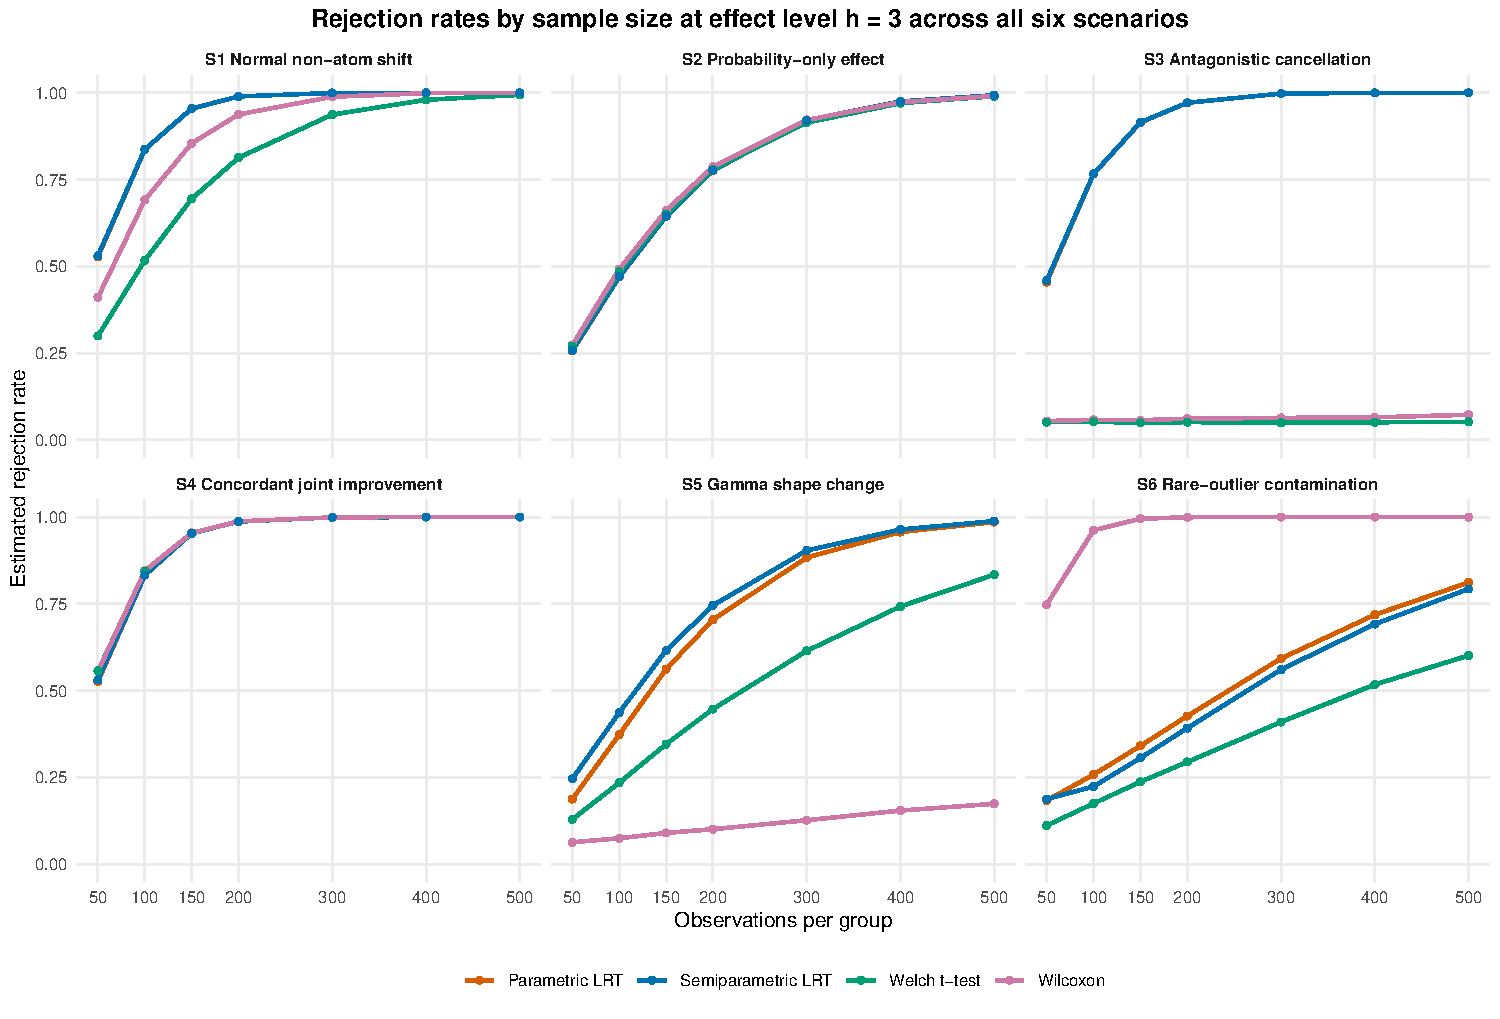
\includegraphics[width=0.84\textwidth]{power-curves.pdf}
\caption{Estimated rejection rates as a function of sample size at effect level $h=3$ for Scenarios~1 through~6.}
\label{fig:powerCurves}
\end{figure}

\begin{figure}[htbp]
\centering
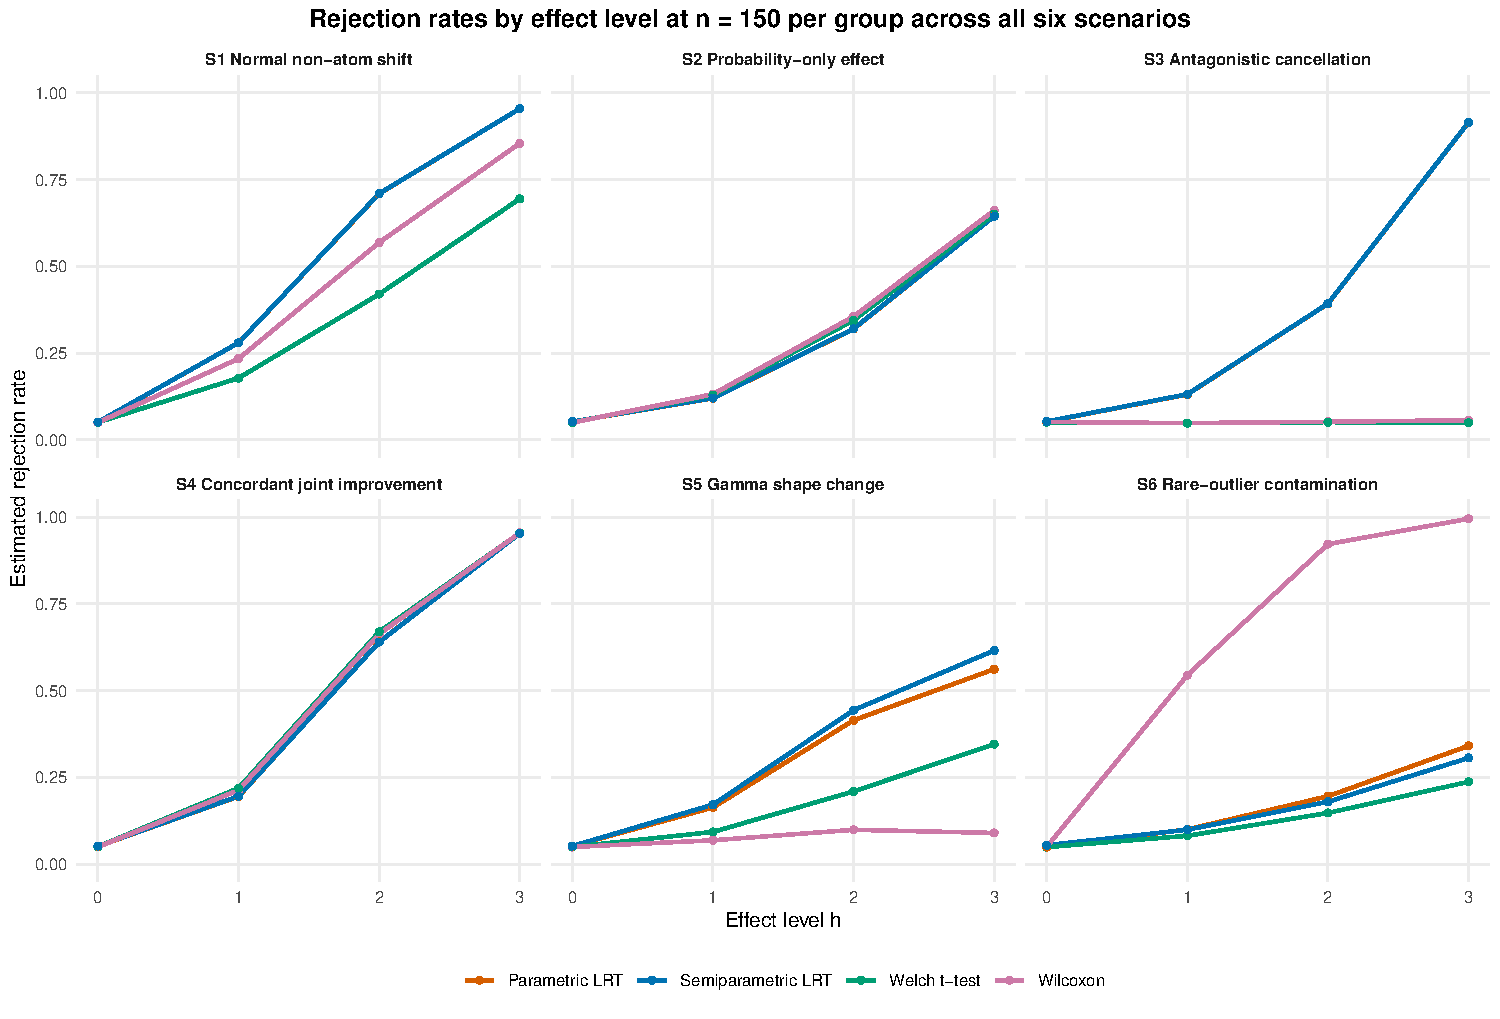
\includegraphics[width=0.84\textwidth]{power-effects.pdf}
\caption{Estimated rejection rates as a function of effect level at $n_{\mathrm{arm}}=150$ observations per arm for Scenarios~1 through~6.}
\label{fig:powerEffectCurves}
\end{figure}
\FloatBarrier

Rejection rates varied across scenarios. In Scenario~1, the Normal non-atom location-shift reference case, the parametric and semiparametric likelihood ratio tests each rejected 95.4\% of replicates at $h=3$ and $n_{\mathrm{arm}}=150$, compared with 85.4\% for Wilcoxon and 69.4\% for Welch's $t$-test. In Scenario~2, where the groups differed only in the probability of being outside the atom, Wilcoxon rejected 66.1\% of replicates and either likelihood ratio test rejected 64.4\% at the same cell, with all four rejection rates near 99\% by $n_{\mathrm{arm}}=500$.

Scenario~3 illustrates the distinction between estimands most directly. The atom-coded marginal mean contrast $\Delta^{(0)}$ is zero at every effect level even though the two-component null is false for $h>0$. At $h=3$ and $n_{\mathrm{arm}}=150$, the likelihood ratio tests rejected about 91.5\% of replicates, whereas Welch's test remained near its nominal rejection rate, as expected under its coded-mean null; the Wilcoxon rejection rate was also near nominal for this configuration. These results reflect different null hypotheses, not a power advantage for a common estimand. By $n_{\mathrm{arm}}=500$, both likelihood ratio tests rejected every replicate, while the coded analyses continued to reject infrequently. In Scenario~4, all four procedures had similar rejection rates.

Scenarios~5 and~6 produced contrasting rejection patterns. In Scenario~5, where the non-atom distribution changed in both shape and mean, the rejection rates at $h=3$ and $n_{\mathrm{arm}}=150$ were 61.5\%, 56.2\%, 34.6\%, and 9.0\% for the semiparametric likelihood ratio test, parametric likelihood ratio test, Welch's $t$-test, and Wilcoxon test, respectively. In Scenario~6, which used rare outlier contamination, the corresponding rejection rates were 30.6\%, 34.1\%, 23.7\%, and 99.5\%. These differences reflect both the simulated distributions and the distinct targets of the procedures.

Null calibration was mostly close to nominal and all method failure rates were zero. The main exception was the semiparametric likelihood ratio test in the null setting with rare outliers. Its rejection rate was 12.6\% at $n_{\mathrm{arm}}=50$ and 6.6\% at $n_{\mathrm{arm}}=100$ before approaching the nominal level from $n_{\mathrm{arm}}\geq150$. The $\chi^2_2$ approximation can converge slowly in this setting because a few extreme observations dominate the empirical-likelihood mean constraint and produce highly uneven weights in small samples. Rejection rates from very small contaminated samples therefore require caution for the semiparametric procedure. In settings with sparse extreme observations, the semiparametric $\chi^2_2$ calibration should be checked before use with fewer than 150 observations per arm.

\section{Application to the IST-3 stroke trial}\label{sec:application}

We applied the proposed methods to \ApplicationDatasetDescription{} \citep{IST3Lancet2012,IST3DataShare}. The application illustrates component-separated endpoint description, one joint frequentist comparison, coded scale summaries, and a Bayesian analysis of the two-part law. Acute ischemic stroke is a natural setting because treatment may affect both mortality and functional health, while death before follow-up is a terminal state rather than a missing quality-of-life value. Among participants alive at six months with observed EQ-VAS, the EuroQol visual analogue score is measured on a 0--100 scale, with larger values indicating better self-rated health.

We obtained the IST-3 data from Edinburgh DataShare under its Data Use Agreement \citep{IST3DataShare}. The fixed-width data and accompanying SAS syntax identified allocated treatment, death by six months, and six-month EQ-VAS\@. We verified the treatment coding against the text treatment field. All analyses use $R=1$ for rt-PA and $R=0$ for placebo or control.

Participants who were alive at six months but had missing EQ-VAS were excluded, while deaths were retained as the atom. The 302 participants who were alive at six months but lacked EQ-VAS were neither deaths nor members of another structural state. They were excluded because this application uses a complete-case outcome analysis. Consequently, all endpoint probabilities and odds below refer to the complete-case endpoint sample comprising deaths and participants alive with observed EQ-VAS\@. The complete-case death proportions exceed the full randomized mortality proportions because excluding survivors with missing EQ-VAS reduces the denominator while leaving the number of deaths unchanged. Within this sample, $A=1$ indicates alive at six months with observed EQ-VAS and $A=0$ denotes death by six months. Let $Y=Y^{\mathrm{EQVAS}}$ when $A=1$. We use the atom code $e_0=-1$, so
\[
  \widetilde{Y}^{(-1)}
  =
  \begin{cases}
    Y, & A=1,\\
    -1, & A=0.
  \end{cases}
\]
Because the non-atom support is contained in $[0,100]$, the coded value $-1$ identifies the atom. The resulting analysis sample included \ApplicationN{} participants, with \ApplicationControlN{} assigned to placebo or control and \ApplicationTreatmentN{} assigned to rt-PA\@. Table~\ref{tab:ist3-descriptives} reports the analysis sample, death counts, EQ-VAS summaries among non-atom observations, and the mean of $\widetilde{Y}^{(-1)}$.

\input{build/tables/application-descriptives.tex}

Figure~\ref{fig:application} displays the atom/non-atom decomposition together with the semiparametric joint confidence region. The proportions of deaths in the complete-case endpoint sample were nearly identical across arms, while EQ-VAS among non-atom observations was higher in the rt-PA arm. The estimated non-atom mean contrast was $\widehat{\mu}_\delta=\ApplicationMuDelta{}$ points. The fitted rt-PA--control odds ratio for being alive with observed EQ-VAS rather than dead within this sample was $\widehat{\alpha}_\delta=\ApplicationAlphaDelta{}$, and the coded scale contrast was $\widehat{\Delta}^{(-1)}=\ApplicationDelta{}$.

\begin{figure}[htbp]
\centering

\includegraphics[width=\textwidth]{application.pdf}
\caption{IST-3 endpoint decomposition and semiparametric likelihood ratio region in the complete-case endpoint sample. The left panel shows deaths and participants alive with observed EQ-VAS by treatment arm. The middle panel shows the EQ-VAS distribution among participants alive with observed scores. The right panel shows the semiparametric likelihood ratio surface for $(\mu_\delta,\log\alpha_\delta)$ with reference lines at $\mu_\delta=0$ and $\log\alpha_\delta=0$. The contours delimit 50\%, 80\%, 95\%, and 99\% likelihood ratio confidence regions, and the solid point marks the unrestricted estimate.}
\label{fig:application}
\end{figure}

Table~\ref{tab:ist3-frequentist} compares standard one-dimensional analyses with the proposed joint tests. Applied to $\widetilde{Y}^{(-1)}$, the Welch $t$-test and Wilcoxon rank-sum test gave $p$-values \ApplicationTTestP{} and \ApplicationWilcoxP{}, respectively. These coded analyses keep deaths in the comparison, but they collapse the endpoint to one dimension. Welch depends on the numerical death code, whereas Wilcoxon treats all deaths as tied observations below the EQ-VAS scores. Analyses restricted to participants alive with observed EQ-VAS gave smaller $p$-values for the EQ-VAS difference, but they condition on the post-randomization event $A=1$ and therefore answer a different observed data question.

\input{build/tables/application-frequentist.tex}

The likelihood ratio procedures test the joint null $\mu_\delta=0$ and $\beta_\delta=0$. Within the complete-case endpoint sample, these restrictions specify no arm difference in the non-atom EQ-VAS mean and no arm difference in the odds of being alive with observed EQ-VAS rather than dead. The parametric likelihood ratio statistic was \ApplicationLRTStatistic{} with $p$-value \ApplicationLRTP{}, and the semiparametric statistic was \ApplicationSPLRTStatistic{} with $p$-value \ApplicationSPLRTP{}. The two statistics were nearly identical in this dataset. The component estimates show that the joint result is driven mainly by the non-atom EQ-VAS mean contrast rather than the atom component.

All three coded mean intervals used a 95\% confidence level. For $\Delta^{(-1)}$, the direct Welch interval was $[\ApplicationDeltaWelchLower{}, \ApplicationDeltaWelchUpper{}]$. The semiparametric profile likelihood interval treating $\Delta^{(-1)}$ as the scalar target was $[\ApplicationDeltaProfileLower{}, \ApplicationDeltaProfileUpper{}]$. Projecting the full four-parameter semiparametric likelihood region onto the $\Delta^{(-1)}$ scale gave the wider interval $[\ApplicationDeltaProjectedLower{}, \ApplicationDeltaProjectedUpper{}]$, reflecting simultaneous uncertainty in both arm means and both atom probabilities.

As an alternative model-based analysis, we specified an application-specific ordered finite mixture with two bounded reported score logit-normal components. Two components allow a bimodal non-atom score distribution while retaining a parsimonious application model. The likelihood was the reported score likelihood in Section~\ref{sec:bayesian-two-group}. The component locations in each arm satisfied $\mu_{r1}<\mu_{r2}$. Independently between arms, their joint prior density on the ordered region was proportional to the product of two $N(0,2^2)$ densities. The mixture weights were $(v_{r1},1-v_{r1})$, with $v_{r1}\mid\tau_r\sim\Beta(1,\tau_r)$ and the first weight attached to the lower location. Independently by arm, $\rho_r\sim\Beta(1,1)$, $\tau_r\sim\mathrm{Gamma}(4,4)$ under the shape--rate convention, and $\log\sigma_{rh}\sim N(\log(1.2),0.5^2)$. A common reporting grid weight vector for widths 1, 5, and 10 had a $\mathrm{Dirichlet}(2,2,2)$ prior. The weights were shared because the score recording mechanism was common to both randomized arms. Four chains used 1{,}000 warmup iterations and 2{,}000 sampling iterations each. Posterior sampling used the No-U-Turn Sampler with a target acceptance probability of 0.995 and a maximum tree depth of 12 \citep{hoffman2014nuts}. There were no divergent transitions, and no transitions reached the maximum tree depth. Across all sampled scalar model parameters, the maximum $\widehat{R}$ was \ApplicationBayesMaxRhat\ and the minimum bulk and tail effective sample sizes were \ApplicationBayesMinBulkEss\ and \ApplicationBayesMinTailEss. The prevalence of rounded scores motivated the reporting grid layer. Among participants alive with observed EQ-VAS, 85.3\% of placebo or control scores and 83.8\% of rt-PA scores were multiples of 5. The corresponding proportions for multiples of 10 were 64.3\% and 62.7\%.

The posterior summaries use corresponding component and coded scale functionals.
At each posterior draw, the fitted non-atom score
probabilities give the arm-specific means $\mu_r^c$, and we form
\[
  \Delta_{\mathrm{atom}}=\rho_1-\rho_0,
  \qquad
  \mu_\delta=\mu_1^c-\mu_0^c,
  \qquad
  \alpha_\delta
  =
  \frac{\pi_1/(1-\pi_1)}{\pi_0/(1-\pi_0)},
  \qquad
  \Delta^{(-1)}
  =
  (-\rho_1+\pi_1\mu_1^c)
  -
  (-\rho_0+\pi_0\mu_0^c).
\]
Table~\ref{tab:ist3-bayes} reports posterior medians, 95\% equal-tailed credible
intervals, and posterior probabilities for the displayed favorable directions.

\input{build/tables/application-bayes-summary.tex}

The posterior summaries reinforce the frequentist decomposition. They give high posterior probability to a positive non-atom EQ-VAS contrast, $\Prob(\mu_\delta>0\mid\mathcal{D}_n)=\ApplicationMuBenefitProbability{}$, little directional evidence that the odds of being alive with observed EQ-VAS were higher under rt-PA, $\Prob(\alpha_\delta>1\mid\mathcal{D}_n)=\ApplicationAlphaBenefitProbability{}$, and substantial posterior probability for a positive coded endpoint contrast, $\Prob(\Delta^{(-1)}>0\mid\mathcal{D}_n)=\ApplicationDeltaBenefitProbability{}$. Figure~\ref{fig:application-posterior} shows the posterior densities for these component and coded scale contrasts.

\begin{figure}[htbp]
\centering

\includegraphics[width=0.92\textwidth]{application-posterior.pdf}
\caption{Posterior distributions for the IST-3 between-arm contrasts. Vertical dashed lines mark no non-atom mean difference, no difference in the odds of being alive with observed EQ-VAS, and no coded endpoint mean difference.}
\label{fig:application-posterior}
\end{figure}

Finally, component-specific posterior predictive checks did not indicate a strong mismatch for either part of the Bayesian model. Among 200 posterior predictive draws, 109 gave an atom-rate discrepancy at least as large as observed and 65 gave a CDF discrepancy for the reported scores at least as large as observed. The corresponding posterior predictive $p$-values were 0.55 and 0.33. These are model checks rather than calibrated classical $p$-values. With 200 replications, the Monte Carlo standard error of a posterior predictive $p$-value is at most 0.035, which is adequate for detecting gross lack of fit but not for estimating small tail probabilities precisely. Appendix~\ref{app:bayesian-ppc} defines both discrepancies, and Figure~\ref{fig:application-ppc} displays the checks.

\begin{figure}[H]
\centering

\includegraphics[width=\textwidth]{application-ppc.pdf}
\caption{Posterior predictive checks for the IST-3 Bayesian model, separately for the death atom and the non-atom EQ-VAS component. Gray bars show observed proportions and black points with vertical ranges show posterior predictive means and 95\% intervals. The left panel uses the death indicator by arm, whereas the right panel uses reported score probability masses among participants alive with observed EQ-VAS\@. The displayed posterior predictive $p$-values are based on component-specific discrepancies for the arm-specific death probabilities and non-atom reported score distributions.}
\label{fig:application-ppc}
\end{figure}


\section{Discussion}\label{sec:discussion}

Building on classical two-part tests that combine evidence from an atom probability and a conditional non-atom response \citep{lachenbruch1976clumping,lachenbruch2001comparisons,lachenbruch2002excess}, we developed parametric and semiparametric likelihood ratio formulations and a Bayesian mixture analysis for outcomes whose observed data law has a substantive atom and a non-atom component. Each frequentist criterion separates exactly into a Bernoulli component for the non-atom probability and a component for the conditional non-atom mean. Under the stated method-specific large-sample conditions, each joint statistic has a $\chi^2_2$ null limit. The tests impose the joint null $\mu_\delta=\beta_\delta=0$, which specifies no between-arm difference in either prespecified component. The framework yields one $p$-value while reporting component estimates, likelihood ratio confidence regions, and summaries on a chosen coded numerical scale. The Bayesian mixture provides a model-based analysis of the full arm-specific observed data laws, with posterior summaries and posterior predictive checks.

The two-component formulation matters because assigning the atom a numerical code, or ranking it below all non-atom values, turns a two-part outcome into a scalar representation. Such analyses may be appropriate for a particular composite endpoint, but they answer a question tied to that representation. The coded mean depends on the numerical atom code, and the rank analysis depends on the chosen ordering. When the components move in opposite directions, a coded mean contrast or a rank-based comparison can be attenuated, or even show little signal, despite component-level differences. The proposed tests retain the atom/non-atom structure while still providing a single prespecified test of the joint null.

Categorical covariate adjustment is an especially favorable case for the semiparametric procedure. With finitely many well-populated joint strata, saturated stratum indicators give a fully nonparametric null model apart from the two component restrictions being tested. The nuisance probabilities and conditional means may vary freely across strata, and the conditional non-atom distributions remain unrestricted subject to the stated moment and regularity conditions. This robustness does not remove the common-contrast interpretation under the alternative. The conditional log odds ratio and conditional non-atom mean difference are assumed to be common across strata, which preserves the two-degree-of-freedom formulation.

The simulation study illustrates how procedures targeting different null hypotheses respond to the same data-generating configurations. In Scenario~3, the component null was false while the atom-coded marginal mean null remained true; the high rejection rate of the likelihood ratio tests and near-nominal rejection rate of Welch's test therefore reflect distinct estimands, not comparative power for a common hypothesis. Across the remaining scenarios, rejection rates varied according to whether the simulated change was visible in the component, coded-mean, or rank-based target. These results should not be read as ranking methods by power for a shared estimand. Null calibration was generally close to nominal, although the semiparametric likelihood ratio test was anti-conservative in the smallest null settings with rare outliers before improving with sample size.

Several limitations follow directly from the construction. The frequentist calibration is asymptotic and requires adequate information in both components, including non-atom observations in both treatment arms. The parametric test requires a correct conditional mean and common conditional variance in addition to the Bernoulli model and regularity conditions. A Gaussian conditional law is sufficient but not necessary. The semiparametric empirical likelihood version removes the common-variance and distributional-shape requirements, but still depends on the Bernoulli model, the conditional mean model, feasible empirical likelihood constraints, and regular nuisance profiling. Likelihood-based coded scale intervals additionally require the expansion and localization in Assumption~\ref{ass:delta-full-lr}. In the IST-3 application, participants who were alive at six months but had missing EQ-VAS were excluded rather than represented through an additional missing-data process or outcome state. The reported non-atom probabilities therefore pertain to the complete-case endpoint sample. The Bayesian analysis was unadjusted and depends on the number of retained mixture components, kernel family, prior choices, and reporting grid model. More generally, the frequentist targets are observed data component contrasts rather than latent causal effects in a principal stratum. The Bayesian target is the full arm-specific observed data law.

These limitations do not remove the practical motivation for the decomposition. When a trial endpoint contains a substantive atom but still requires one primary comparison, the proposed likelihood ratio tests and the Bayesian alternative give a way to keep the atom probability and the non-atom outcome visible in the same analysis. The aim is not to replace every coded or ranked composite, but to make clear when such a composite is hiding clinically relevant component behavior.

\section*{Funding}
The authors received no specific funding for this work.

\section*{Conflict of interest}
The authors declare no conflicts of interest.

\section*{Author contributions}
Andreas Kryger Jensen: Conceptualization, methodology, software, formal
analysis, visualization, and writing original draft. Theis Lange: Conceptualization, methodology, and editing.

\section*{Acknowledgments}
We acknowledge the data custodian, Peter Sandercock on behalf of the IST-3 Collaborative Group. We gratefully acknowledge the IST-3 Collaborative Group, the trial joint sponsors (The University of Edinburgh and the Lothian Health Board), and the chief funding agencies of the study: UK Medical Research Council, Health Foundation UK, Stroke Association UK, Research Council of Norway, Arbetsmarknadens Partners Forsakringsbolag (AFA) Insurances Sweden, Swedish Heart Lung Fund, The Foundation of Marianne and Marcus Wallenberg, Polish Ministry of Science and Education, the Australian Heart Foundation, Australian National Health and Medical Research Council (NHMRC), Swiss National Research Foundation, Swiss Heart Foundation, Assessorato alla Sanita, Regione dell'Umbria, Italy, and Danube University.

\fi

\ifManuscriptIncludeSupplement
\clearpage
\appendix
\ifProofsExternal
\section{Proofs for main text results}\label{app:main-text-proofs}
\includeExternalAppendix[mainproofs]{two_component_treatment_comparisons_main}
\else\ifProofsToAppendix
\section{Proofs for main text results}\label{app:main-text-proofs}
\printProofs[mainproofs]
\fi
\fi
\section{Supplementary simulation results}\label{app:supplementary-simulation-results}

This appendix gives additional design details for the simulation study in Section~\ref{sec:simulation-study} and reports the full numerical rejection rates underlying the main text figures.

For each cell defined by scenario, effect level, and sample size, the random-number seed was set to $20260416$ plus the cell index minus one. Cells were ordered by scenario, then effect level, then sample size. Sample size varied fastest within each combination of scenario and effect level. Each cell used 25,000 Monte Carlo repetitions. Each replicate was analyzed using the Wilcoxon rank-sum test, Welch's two-sample $t$-test, the parametric likelihood ratio test, and the semiparametric likelihood ratio test. Rejection was recorded when the method returned a finite $p$-value below $0.05$. A method failure was recorded when the method did not return a finite $p$-value.

Figure~\ref{fig:type1Curves} gives the full null calibration display for the $h=0$ cells. The figure and tables report rejection percentages for 5\% tests. In the scenario tables, $h=0$ rows assess the common null configuration and $h>0$ rows report rejection percentages under the displayed data-generating configurations. Because the procedures generally target different null hypotheses, the latter are not power comparisons for a common estimand. LRT and SPLRT denote the parametric and semiparametric likelihood ratio tests. The column ``Expected $\Delta^{(0)}$'' is the expected coded mean contrast for atom code $e_0=0$.

\begin{figure}[htbp]
\centering
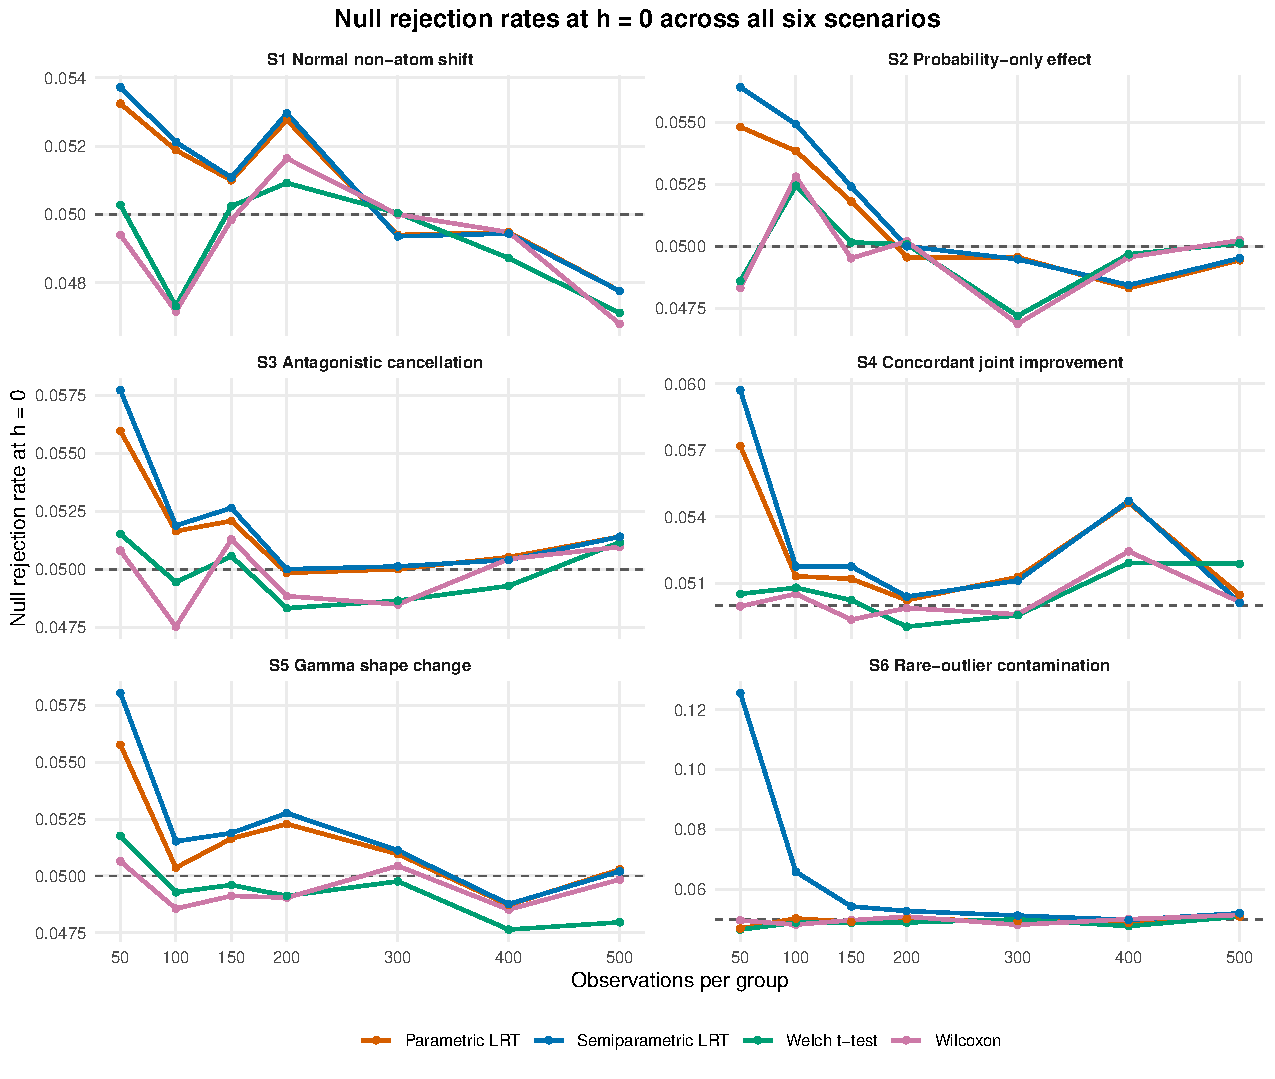
\includegraphics[width=0.84\textwidth]{type1-curves.pdf}
\caption{Null rejection rates at effect level $h = 0$ across all six simulation scenarios. The dashed line marks 0.05.}
\label{fig:type1Curves}
\end{figure}

\begingroup\fontsize{7}{9}\selectfont

\begin{longtable}[t]{rrlrrrrr}
\caption{Scenario S1 (Normal non-atom shift, low atom probability): estimated rejection percentages by sample size and effect level}\\
\toprule
$n_{\mathrm{arm}}$ & $h$ & Effect & Expected $\Delta^{(0)}$ & Wilcoxon (\%) & Welch $t$-test (\%) & LRT (\%) & SPLRT (\%)\\
\midrule
\endfirsthead
\caption[]{Scenario S1 (Normal non-atom shift, low atom probability): estimated rejection percentages by sample size and effect level \textit{(continued)}}\\
\toprule
$n_{\mathrm{arm}}$ & $h$ & Effect & Expected $\Delta^{(0)}$ & Wilcoxon (\%) & Welch $t$-test (\%) & LRT (\%) & SPLRT (\%)\\
\midrule
\endhead

\endfoot
\bottomrule
\endlastfoot
50 & 0 & \makecell[l]{$\delta_h = 0.00$} & 0.000 & 4.94 & 5.03 & 5.32 & 5.37\\
100 & 0 & \makecell[l]{$\delta_h = 0.00$} & 0.000 & 4.72 & 4.73 & 5.19 & 5.21\\
150 & 0 & \makecell[l]{$\delta_h = 0.00$} & 0.000 & 4.98 & 5.02 & 5.10 & 5.11\\
200 & 0 & \makecell[l]{$\delta_h = 0.00$} & 0.000 & 5.16 & 5.09 & 5.28 & 5.30\\
300 & 0 & \makecell[l]{$\delta_h = 0.00$} & 0.000 & 5.00 & 5.00 & 4.94 & 4.94\\
400 & 0 & \makecell[l]{$\delta_h = 0.00$} & 0.000 & 4.95 & 4.87 & 4.95 & 4.94\\
500 & 0 & \makecell[l]{$\delta_h = 0.00$} & 0.000 & 4.68 & 4.71 & 4.78 & 4.78\\
50 & 1 & \makecell[l]{$\delta_h = 0.20$} & 0.170 & 10.65 & 9.25 & 12.44 & 12.56\\
100 & 1 & \makecell[l]{$\delta_h = 0.20$} & 0.170 & 16.89 & 13.26 & 20.16 & 20.17\\
150 & 1 & \makecell[l]{$\delta_h = 0.20$} & 0.170 & 23.37 & 17.78 & 27.97 & 27.97\\
200 & 1 & \makecell[l]{$\delta_h = 0.20$} & 0.170 & 29.32 & 21.86 & 35.98 & 36.01\\
300 & 1 & \makecell[l]{$\delta_h = 0.20$} & 0.170 & 40.84 & 30.20 & 50.76 & 50.78\\
400 & 1 & \makecell[l]{$\delta_h = 0.20$} & 0.170 & 52.36 & 39.04 & 64.54 & 64.60\\
500 & 1 & \makecell[l]{$\delta_h = 0.20$} & 0.170 & 60.72 & 45.90 & 74.45 & 74.40\\
50 & 2 & \makecell[l]{$\delta_h = 0.35$} & 0.298 & 22.98 & 17.55 & 28.78 & 29.02\\
100 & 2 & \makecell[l]{$\delta_h = 0.35$} & 0.298 & 41.03 & 30.20 & 51.88 & 52.00\\
150 & 2 & \makecell[l]{$\delta_h = 0.35$} & 0.298 & 56.84 & 41.98 & 70.91 & 70.96\\
200 & 2 & \makecell[l]{$\delta_h = 0.35$} & 0.298 & 69.77 & 53.36 & 83.26 & 83.22\\
300 & 2 & \makecell[l]{$\delta_h = 0.35$} & 0.298 & 85.27 & 69.76 & 95.02 & 95.03\\
400 & 2 & \makecell[l]{$\delta_h = 0.35$} & 0.298 & 93.56 & 81.58 & 98.80 & 98.80\\
500 & 2 & \makecell[l]{$\delta_h = 0.35$} & 0.298 & 97.37 & 89.66 & 99.76 & 99.76\\
50 & 3 & \makecell[l]{$\delta_h = 0.50$} & 0.425 & 41.04 & 29.95 & 52.75 & 53.05\\
100 & 3 & \makecell[l]{$\delta_h = 0.50$} & 0.425 & 69.14 & 51.71 & 83.67 & 83.70\\
150 & 3 & \makecell[l]{$\delta_h = 0.50$} & 0.425 & 85.45 & 69.44 & 95.45 & 95.44\\
200 & 3 & \makecell[l]{$\delta_h = 0.50$} & 0.425 & 93.76 & 81.30 & 98.95 & 98.95\\
300 & 3 & \makecell[l]{$\delta_h = 0.50$} & 0.425 & 98.86 & 93.72 & 99.94 & 99.94\\
400 & 3 & \makecell[l]{$\delta_h = 0.50$} & 0.425 & 99.88 & 97.97 & 100.00 & 100.00\\
500 & 3 & \makecell[l]{$\delta_h = 0.50$} & 0.425 & 99.98 & 99.40 & 100.00 & 100.00\\*
\end{longtable}
\endgroup{}

\begingroup\fontsize{7}{9}\selectfont

\begin{longtable}[t]{rrlrrrrr}
\caption{Scenario S2 (effect only on probability outside atom): estimated rejection percentages by sample size and effect level}\\
\toprule
$n_{\mathrm{arm}}$ & $h$ & Effect & Expected $\Delta^{(0)}$ & Wilcoxon (\%) & Welch $t$-test (\%) & LRT (\%) & SPLRT (\%)\\
\midrule
\endfirsthead
\caption[]{Scenario S2 (effect only on probability outside atom): estimated rejection percentages by sample size and effect level \textit{(continued)}}\\
\toprule
$n_{\mathrm{arm}}$ & $h$ & Effect & Expected $\Delta^{(0)}$ & Wilcoxon (\%) & Welch $t$-test (\%) & LRT (\%) & SPLRT (\%)\\
\midrule
\endhead

\endfoot
\bottomrule
\endlastfoot
50 & 0 & \makecell[l]{$\pi_{1,h} = 0.45$} & 0.00 & 4.83 & 4.86 & 5.48 & 5.64\\
100 & 0 & \makecell[l]{$\pi_{1,h} = 0.45$} & 0.00 & 5.28 & 5.24 & 5.38 & 5.49\\
150 & 0 & \makecell[l]{$\pi_{1,h} = 0.45$} & 0.00 & 4.95 & 5.02 & 5.18 & 5.24\\
200 & 0 & \makecell[l]{$\pi_{1,h} = 0.45$} & 0.00 & 5.02 & 5.01 & 4.96 & 5.00\\
300 & 0 & \makecell[l]{$\pi_{1,h} = 0.45$} & 0.00 & 4.69 & 4.72 & 4.96 & 4.95\\
400 & 0 & \makecell[l]{$\pi_{1,h} = 0.45$} & 0.00 & 4.96 & 4.97 & 4.83 & 4.84\\
500 & 0 & \makecell[l]{$\pi_{1,h} = 0.45$} & 0.00 & 5.02 & 5.01 & 4.94 & 4.95\\
50 & 1 & \makecell[l]{$\pi_{1,h} = 0.50$} & 0.15 & 7.70 & 7.74 & 7.74 & 7.91\\
100 & 1 & \makecell[l]{$\pi_{1,h} = 0.50$} & 0.15 & 9.90 & 9.76 & 9.04 & 9.04\\
150 & 1 & \makecell[l]{$\pi_{1,h} = 0.50$} & 0.15 & 13.13 & 12.89 & 11.96 & 12.01\\
200 & 1 & \makecell[l]{$\pi_{1,h} = 0.50$} & 0.15 & 15.28 & 14.79 & 13.08 & 13.09\\
300 & 1 & \makecell[l]{$\pi_{1,h} = 0.50$} & 0.15 & 20.23 & 19.51 & 17.86 & 17.88\\
400 & 1 & \makecell[l]{$\pi_{1,h} = 0.50$} & 0.15 & 26.26 & 25.10 & 22.88 & 22.90\\
500 & 1 & \makecell[l]{$\pi_{1,h} = 0.50$} & 0.15 & 31.61 & 30.40 & 27.64 & 27.64\\
50 & 2 & \makecell[l]{$\pi_{1,h} = 0.55$} & 0.30 & 14.73 & 14.51 & 13.93 & 14.15\\
100 & 2 & \makecell[l]{$\pi_{1,h} = 0.55$} & 0.30 & 25.27 & 24.69 & 23.11 & 23.11\\
150 & 2 & \makecell[l]{$\pi_{1,h} = 0.55$} & 0.30 & 35.54 & 34.42 & 31.94 & 31.98\\
200 & 2 & \makecell[l]{$\pi_{1,h} = 0.55$} & 0.30 & 45.40 & 43.97 & 41.52 & 41.54\\
300 & 2 & \makecell[l]{$\pi_{1,h} = 0.55$} & 0.30 & 61.90 & 60.21 & 58.91 & 58.90\\
400 & 2 & \makecell[l]{$\pi_{1,h} = 0.55$} & 0.30 & 74.22 & 72.58 & 71.88 & 71.86\\
500 & 2 & \makecell[l]{$\pi_{1,h} = 0.55$} & 0.30 & 83.02 & 81.57 & 81.38 & 81.39\\
50 & 3 & \makecell[l]{$\pi_{1,h} = 0.60$} & 0.45 & 27.30 & 27.02 & 25.59 & 25.84\\
100 & 3 & \makecell[l]{$\pi_{1,h} = 0.60$} & 0.45 & 49.18 & 48.44 & 46.92 & 47.00\\
150 & 3 & \makecell[l]{$\pi_{1,h} = 0.60$} & 0.45 & 66.08 & 64.98 & 64.40 & 64.39\\
200 & 3 & \makecell[l]{$\pi_{1,h} = 0.60$} & 0.45 & 78.67 & 77.90 & 77.57 & 77.59\\
300 & 3 & \makecell[l]{$\pi_{1,h} = 0.60$} & 0.45 & 92.17 & 91.39 & 92.10 & 92.10\\
400 & 3 & \makecell[l]{$\pi_{1,h} = 0.60$} & 0.45 & 97.29 & 97.01 & 97.50 & 97.50\\
500 & 3 & \makecell[l]{$\pi_{1,h} = 0.60$} & 0.45 & 99.09 & 99.00 & 99.30 & 99.30\\*
\end{longtable}
\endgroup{}

\begingroup\fontsize{7}{9}\selectfont

\begin{longtable}[t]{rrlrrrrr}
\caption{Scenario S3 (antagonistic cancellation): estimated rejection percentages by sample size and effect level}\\
\toprule
$n_{\mathrm{arm}}$ & $h$ & Effect & Expected $\Delta^{(0)}$ & Wilcoxon (\%) & Welch $t$-test (\%) & LRT (\%) & SPLRT (\%)\\
\midrule
\endfirsthead
\caption[]{Scenario S3 (antagonistic cancellation): estimated rejection percentages by sample size and effect level \textit{(continued)}}\\
\toprule
$n_{\mathrm{arm}}$ & $h$ & Effect & Expected $\Delta^{(0)}$ & Wilcoxon (\%) & Welch $t$-test (\%) & LRT (\%) & SPLRT (\%)\\
\midrule
\endhead

\endfoot
\bottomrule
\endlastfoot
50 & 0 & \makecell[l]{$\pi_{1,h} = 0.500$, $1.5 / \pi_{1,h} = 3.000$} & 0 & 5.08 & 5.15 & 5.60 & 5.77\\
100 & 0 & \makecell[l]{$\pi_{1,h} = 0.500$, $1.5 / \pi_{1,h} = 3.000$} & 0 & 4.75 & 4.94 & 5.16 & 5.19\\
150 & 0 & \makecell[l]{$\pi_{1,h} = 0.500$, $1.5 / \pi_{1,h} = 3.000$} & 0 & 5.13 & 5.06 & 5.21 & 5.26\\
200 & 0 & \makecell[l]{$\pi_{1,h} = 0.500$, $1.5 / \pi_{1,h} = 3.000$} & 0 & 4.88 & 4.83 & 4.98 & 5.00\\
300 & 0 & \makecell[l]{$\pi_{1,h} = 0.500$, $1.5 / \pi_{1,h} = 3.000$} & 0 & 4.85 & 4.86 & 5.00 & 5.01\\
400 & 0 & \makecell[l]{$\pi_{1,h} = 0.500$, $1.5 / \pi_{1,h} = 3.000$} & 0 & 5.04 & 4.93 & 5.05 & 5.04\\
500 & 0 & \makecell[l]{$\pi_{1,h} = 0.500$, $1.5 / \pi_{1,h} = 3.000$} & 0 & 5.10 & 5.12 & 5.14 & 5.14\\
50 & 1 & \makecell[l]{$\pi_{1,h} = 0.525$, $1.5 / \pi_{1,h} = 2.857$} & 0 & 5.10 & 5.16 & 8.12 & 8.39\\
100 & 1 & \makecell[l]{$\pi_{1,h} = 0.525$, $1.5 / \pi_{1,h} = 2.857$} & 0 & 4.92 & 4.94 & 10.43 & 10.46\\
150 & 1 & \makecell[l]{$\pi_{1,h} = 0.525$, $1.5 / \pi_{1,h} = 2.857$} & 0 & 4.81 & 4.80 & 13.06 & 13.12\\
200 & 1 & \makecell[l]{$\pi_{1,h} = 0.525$, $1.5 / \pi_{1,h} = 2.857$} & 0 & 5.01 & 4.99 & 16.37 & 16.44\\
300 & 1 & \makecell[l]{$\pi_{1,h} = 0.525$, $1.5 / \pi_{1,h} = 2.857$} & 0 & 4.90 & 4.86 & 21.46 & 21.48\\
400 & 1 & \makecell[l]{$\pi_{1,h} = 0.525$, $1.5 / \pi_{1,h} = 2.857$} & 0 & 5.15 & 5.03 & 28.53 & 28.52\\
500 & 1 & \makecell[l]{$\pi_{1,h} = 0.525$, $1.5 / \pi_{1,h} = 2.857$} & 0 & 5.08 & 4.99 & 34.50 & 34.49\\
50 & 2 & \makecell[l]{$\pi_{1,h} = 0.550$, $1.5 / \pi_{1,h} = 2.727$} & 0 & 4.74 & 4.92 & 15.72 & 16.10\\
100 & 2 & \makecell[l]{$\pi_{1,h} = 0.550$, $1.5 / \pi_{1,h} = 2.727$} & 0 & 5.33 & 5.22 & 27.74 & 27.78\\
150 & 2 & \makecell[l]{$\pi_{1,h} = 0.550$, $1.5 / \pi_{1,h} = 2.727$} & 0 & 5.19 & 5.06 & 39.20 & 39.23\\
200 & 2 & \makecell[l]{$\pi_{1,h} = 0.550$, $1.5 / \pi_{1,h} = 2.727$} & 0 & 5.12 & 4.99 & 49.88 & 49.83\\
300 & 2 & \makecell[l]{$\pi_{1,h} = 0.550$, $1.5 / \pi_{1,h} = 2.727$} & 0 & 5.51 & 5.10 & 68.10 & 68.15\\
400 & 2 & \makecell[l]{$\pi_{1,h} = 0.550$, $1.5 / \pi_{1,h} = 2.727$} & 0 & 5.60 & 5.09 & 80.76 & 80.78\\
500 & 2 & \makecell[l]{$\pi_{1,h} = 0.550$, $1.5 / \pi_{1,h} = 2.727$} & 0 & 5.56 & 5.10 & 89.15 & 89.10\\
50 & 3 & \makecell[l]{$\pi_{1,h} = 0.600$, $1.5 / \pi_{1,h} = 2.500$} & 0 & 5.41 & 5.06 & 45.44 & 45.90\\
100 & 3 & \makecell[l]{$\pi_{1,h} = 0.600$, $1.5 / \pi_{1,h} = 2.500$} & 0 & 5.71 & 5.20 & 76.60 & 76.64\\
150 & 3 & \makecell[l]{$\pi_{1,h} = 0.600$, $1.5 / \pi_{1,h} = 2.500$} & 0 & 5.65 & 4.88 & 91.47 & 91.49\\
200 & 3 & \makecell[l]{$\pi_{1,h} = 0.600$, $1.5 / \pi_{1,h} = 2.500$} & 0 & 6.06 & 5.08 & 97.12 & 97.12\\
300 & 3 & \makecell[l]{$\pi_{1,h} = 0.600$, $1.5 / \pi_{1,h} = 2.500$} & 0 & 6.32 & 4.93 & 99.78 & 99.78\\
400 & 3 & \makecell[l]{$\pi_{1,h} = 0.600$, $1.5 / \pi_{1,h} = 2.500$} & 0 & 6.46 & 5.04 & 99.97 & 99.97\\
500 & 3 & \makecell[l]{$\pi_{1,h} = 0.600$, $1.5 / \pi_{1,h} = 2.500$} & 0 & 7.22 & 5.14 & 100.00 & 100.00\\*
\end{longtable}
\endgroup{}

\begingroup\fontsize{7}{9}\selectfont

\begin{longtable}[t]{rrlrrrrr}
\caption{Scenario S4 (concordant joint improvement): estimated rejection percentages by sample size and effect level}\\
\toprule
$n_{\mathrm{arm}}$ & $h$ & Effect & Expected $\Delta^{(0)}$ & Wilcoxon (\%) & Welch $t$-test (\%) & LRT (\%) & SPLRT (\%)\\
\midrule
\endfirsthead
\caption[]{Scenario S4 (concordant joint improvement): estimated rejection percentages by sample size and effect level \textit{(continued)}}\\
\toprule
$n_{\mathrm{arm}}$ & $h$ & Effect & Expected $\Delta^{(0)}$ & Wilcoxon (\%) & Welch $t$-test (\%) & LRT (\%) & SPLRT (\%)\\
\midrule
\endhead

\endfoot
\bottomrule
\endlastfoot
50 & 0 & \makecell[l]{$\pi_{1,h} = 0.50$, $3 + 0.15h = 3.00$} & 0.000 & 5.00 & 5.05 & 5.72 & 5.97\\
100 & 0 & \makecell[l]{$\pi_{1,h} = 0.50$, $3 + 0.15h = 3.00$} & 0.000 & 5.05 & 5.08 & 5.13 & 5.18\\
150 & 0 & \makecell[l]{$\pi_{1,h} = 0.50$, $3 + 0.15h = 3.00$} & 0.000 & 4.94 & 5.02 & 5.12 & 5.18\\
200 & 0 & \makecell[l]{$\pi_{1,h} = 0.50$, $3 + 0.15h = 3.00$} & 0.000 & 4.99 & 4.90 & 5.02 & 5.04\\
300 & 0 & \makecell[l]{$\pi_{1,h} = 0.50$, $3 + 0.15h = 3.00$} & 0.000 & 4.96 & 4.96 & 5.13 & 5.11\\
400 & 0 & \makecell[l]{$\pi_{1,h} = 0.50$, $3 + 0.15h = 3.00$} & 0.000 & 5.24 & 5.19 & 5.46 & 5.47\\
500 & 0 & \makecell[l]{$\pi_{1,h} = 0.50$, $3 + 0.15h = 3.00$} & 0.000 & 5.02 & 5.19 & 5.05 & 5.01\\
50 & 1 & \makecell[l]{$\pi_{1,h} = 0.55$, $3 + 0.15h = 3.15$} & 0.233 & 10.04 & 10.37 & 9.84 & 10.07\\
100 & 1 & \makecell[l]{$\pi_{1,h} = 0.55$, $3 + 0.15h = 3.15$} & 0.233 & 15.71 & 16.25 & 14.39 & 14.47\\
150 & 1 & \makecell[l]{$\pi_{1,h} = 0.55$, $3 + 0.15h = 3.15$} & 0.233 & 21.30 & 21.88 & 19.48 & 19.54\\
200 & 1 & \makecell[l]{$\pi_{1,h} = 0.55$, $3 + 0.15h = 3.15$} & 0.233 & 26.52 & 27.40 & 24.43 & 24.40\\
300 & 1 & \makecell[l]{$\pi_{1,h} = 0.55$, $3 + 0.15h = 3.15$} & 0.233 & 37.70 & 38.72 & 34.90 & 34.93\\
400 & 1 & \makecell[l]{$\pi_{1,h} = 0.55$, $3 + 0.15h = 3.15$} & 0.233 & 48.14 & 49.66 & 45.59 & 45.53\\
500 & 1 & \makecell[l]{$\pi_{1,h} = 0.55$, $3 + 0.15h = 3.15$} & 0.233 & 56.48 & 57.87 & 54.23 & 54.19\\
50 & 2 & \makecell[l]{$\pi_{1,h} = 0.60$, $3 + 0.15h = 3.30$} & 0.480 & 27.45 & 28.01 & 25.71 & 26.04\\
100 & 2 & \makecell[l]{$\pi_{1,h} = 0.60$, $3 + 0.15h = 3.30$} & 0.480 & 48.84 & 49.53 & 46.02 & 46.10\\
150 & 2 & \makecell[l]{$\pi_{1,h} = 0.60$, $3 + 0.15h = 3.30$} & 0.480 & 66.29 & 66.94 & 64.03 & 63.99\\
200 & 2 & \makecell[l]{$\pi_{1,h} = 0.60$, $3 + 0.15h = 3.30$} & 0.480 & 78.16 & 78.66 & 76.47 & 76.44\\
300 & 2 & \makecell[l]{$\pi_{1,h} = 0.60$, $3 + 0.15h = 3.30$} & 0.480 & 91.95 & 92.20 & 91.80 & 91.84\\
400 & 2 & \makecell[l]{$\pi_{1,h} = 0.60$, $3 + 0.15h = 3.30$} & 0.480 & 97.39 & 97.56 & 97.56 & 97.56\\
500 & 2 & \makecell[l]{$\pi_{1,h} = 0.60$, $3 + 0.15h = 3.30$} & 0.480 & 99.20 & 99.27 & 99.33 & 99.33\\
50 & 3 & \makecell[l]{$\pi_{1,h} = 0.65$, $3 + 0.15h = 3.45$} & 0.743 & 55.57 & 55.71 & 52.62 & 53.11\\
100 & 3 & \makecell[l]{$\pi_{1,h} = 0.65$, $3 + 0.15h = 3.45$} & 0.743 & 84.54 & 84.45 & 83.25 & 83.26\\
150 & 3 & \makecell[l]{$\pi_{1,h} = 0.65$, $3 + 0.15h = 3.45$} & 0.743 & 95.45 & 95.40 & 95.32 & 95.32\\
200 & 3 & \makecell[l]{$\pi_{1,h} = 0.65$, $3 + 0.15h = 3.45$} & 0.743 & 98.77 & 98.69 & 98.76 & 98.74\\
300 & 3 & \makecell[l]{$\pi_{1,h} = 0.65$, $3 + 0.15h = 3.45$} & 0.743 & 99.92 & 99.92 & 99.91 & 99.91\\
400 & 3 & \makecell[l]{$\pi_{1,h} = 0.65$, $3 + 0.15h = 3.45$} & 0.743 & 100.00 & 100.00 & 100.00 & 100.00\\
500 & 3 & \makecell[l]{$\pi_{1,h} = 0.65$, $3 + 0.15h = 3.45$} & 0.743 & 100.00 & 100.00 & 100.00 & 100.00\\*
\end{longtable}
\endgroup{}

\begingroup\fontsize{7}{9}\selectfont

\begin{longtable}[t]{rrlrrrrr}
\caption{Scenario S5 (Gamma shape change with non-atom mean shift): estimated rejection percentages by sample size and effect level}\\
\toprule
$n_{\mathrm{arm}}$ & $h$ & Effect & Expected $\Delta^{(0)}$ & Wilcoxon (\%) & Welch $t$-test (\%) & LRT (\%) & SPLRT (\%)\\
\midrule
\endfirsthead
\caption[]{Scenario S5 (Gamma shape change with non-atom mean shift): estimated rejection percentages by sample size and effect level \textit{(continued)}}\\
\toprule
$n_{\mathrm{arm}}$ & $h$ & Effect & Expected $\Delta^{(0)}$ & Wilcoxon (\%) & Welch $t$-test (\%) & LRT (\%) & SPLRT (\%)\\
\midrule
\endhead

\endfoot
\bottomrule
\endlastfoot
50 & 0 & \makecell[l]{$k_h = 9.0$, $m_h = 3.0$} & 0.00 & 5.06 & 5.18 & 5.58 & 5.80\\
100 & 0 & \makecell[l]{$k_h = 9.0$, $m_h = 3.0$} & 0.00 & 4.86 & 4.93 & 5.04 & 5.15\\
150 & 0 & \makecell[l]{$k_h = 9.0$, $m_h = 3.0$} & 0.00 & 4.91 & 4.96 & 5.16 & 5.19\\
200 & 0 & \makecell[l]{$k_h = 9.0$, $m_h = 3.0$} & 0.00 & 4.90 & 4.91 & 5.23 & 5.28\\
300 & 0 & \makecell[l]{$k_h = 9.0$, $m_h = 3.0$} & 0.00 & 5.04 & 4.98 & 5.10 & 5.11\\
400 & 0 & \makecell[l]{$k_h = 9.0$, $m_h = 3.0$} & 0.00 & 4.85 & 4.76 & 4.87 & 4.88\\
500 & 0 & \makecell[l]{$k_h = 9.0$, $m_h = 3.0$} & 0.00 & 4.98 & 4.80 & 5.03 & 5.02\\
50 & 1 & \makecell[l]{$k_h = 6.0$, $m_h = 3.2$} & 0.13 & 5.96 & 6.63 & 8.91 & 9.80\\
100 & 1 & \makecell[l]{$k_h = 6.0$, $m_h = 3.2$} & 0.13 & 6.20 & 7.92 & 12.72 & 13.58\\
150 & 1 & \makecell[l]{$k_h = 6.0$, $m_h = 3.2$} & 0.13 & 6.85 & 9.26 & 16.30 & 17.12\\
200 & 1 & \makecell[l]{$k_h = 6.0$, $m_h = 3.2$} & 0.13 & 8.29 & 11.55 & 21.71 & 22.67\\
300 & 1 & \makecell[l]{$k_h = 6.0$, $m_h = 3.2$} & 0.13 & 9.30 & 14.70 & 30.54 & 31.38\\
400 & 1 & \makecell[l]{$k_h = 6.0$, $m_h = 3.2$} & 0.13 & 11.04 & 18.03 & 40.04 & 40.98\\
500 & 1 & \makecell[l]{$k_h = 6.0$, $m_h = 3.2$} & 0.13 & 12.30 & 21.38 & 48.68 & 49.41\\
50 & 2 & \makecell[l]{$k_h = 4.0$, $m_h = 3.4$} & 0.26 & 6.47 & 9.68 & 15.12 & 18.01\\
100 & 2 & \makecell[l]{$k_h = 4.0$, $m_h = 3.4$} & 0.26 & 8.02 & 14.93 & 27.95 & 31.22\\
150 & 2 & \makecell[l]{$k_h = 4.0$, $m_h = 3.4$} & 0.26 & 9.87 & 20.93 & 41.44 & 44.35\\
200 & 2 & \makecell[l]{$k_h = 4.0$, $m_h = 3.4$} & 0.26 & 11.56 & 26.98 & 52.85 & 55.68\\
300 & 2 & \makecell[l]{$k_h = 4.0$, $m_h = 3.4$} & 0.26 & 14.77 & 38.62 & 72.55 & 74.50\\
400 & 2 & \makecell[l]{$k_h = 4.0$, $m_h = 3.4$} & 0.26 & 18.50 & 48.62 & 84.90 & 86.06\\
500 & 2 & \makecell[l]{$k_h = 4.0$, $m_h = 3.4$} & 0.26 & 22.02 & 58.51 & 92.46 & 93.10\\
50 & 3 & \makecell[l]{$k_h = 2.5$, $m_h = 3.6$} & 0.39 & 6.28 & 12.90 & 18.73 & 24.58\\
100 & 3 & \makecell[l]{$k_h = 2.5$, $m_h = 3.6$} & 0.39 & 7.42 & 23.42 & 37.29 & 43.65\\
150 & 3 & \makecell[l]{$k_h = 2.5$, $m_h = 3.6$} & 0.39 & 8.97 & 34.56 & 56.16 & 61.55\\
200 & 3 & \makecell[l]{$k_h = 2.5$, $m_h = 3.6$} & 0.39 & 10.05 & 44.68 & 70.41 & 74.56\\
300 & 3 & \makecell[l]{$k_h = 2.5$, $m_h = 3.6$} & 0.39 & 12.63 & 61.43 & 88.36 & 90.35\\
400 & 3 & \makecell[l]{$k_h = 2.5$, $m_h = 3.6$} & 0.39 & 15.41 & 74.24 & 95.70 & 96.42\\
500 & 3 & \makecell[l]{$k_h = 2.5$, $m_h = 3.6$} & 0.39 & 17.37 & 83.40 & 98.56 & 98.84\\*
\end{longtable}
\endgroup{}

\begingroup\fontsize{7}{9}\selectfont

\begin{longtable}[t]{rrlrrrrr}
\caption{Scenario S6 (rare outlier contamination): estimated rejection percentages by sample size and effect level}\\
\toprule
$n_{\mathrm{arm}}$ & $h$ & Effect & Expected $\Delta^{(0)}$ & Wilcoxon (\%) & Welch $t$-test (\%) & LRT (\%) & SPLRT (\%)\\
\midrule
\endfirsthead
\caption[]{Scenario S6 (rare outlier contamination): estimated rejection percentages by sample size and effect level \textit{(continued)}}\\
\toprule
$n_{\mathrm{arm}}$ & $h$ & Effect & Expected $\Delta^{(0)}$ & Wilcoxon (\%) & Welch $t$-test (\%) & LRT (\%) & SPLRT (\%)\\
\midrule
\endhead

\endfoot
\bottomrule
\endlastfoot
50 & 0 & \makecell[l]{$\delta_h = 0.00$} & 0.00 & 4.96 & 4.65 & 4.68 & 12.55\\
100 & 0 & \makecell[l]{$\delta_h = 0.00$} & 0.00 & 4.82 & 4.88 & 5.02 & 6.58\\
150 & 0 & \makecell[l]{$\delta_h = 0.00$} & 0.00 & 4.96 & 4.88 & 4.91 & 5.42\\
200 & 0 & \makecell[l]{$\delta_h = 0.00$} & 0.00 & 5.08 & 4.89 & 5.01 & 5.27\\
300 & 0 & \makecell[l]{$\delta_h = 0.00$} & 0.00 & 4.81 & 4.99 & 4.94 & 5.12\\
400 & 0 & \makecell[l]{$\delta_h = 0.00$} & 0.00 & 5.00 & 4.77 & 4.88 & 4.98\\
500 & 0 & \makecell[l]{$\delta_h = 0.00$} & 0.00 & 5.14 & 5.09 & 5.09 & 5.20\\
50 & 1 & \makecell[l]{$\delta_h = 0.15$} & 0.12 & 22.17 & 6.10 & 7.68 & 15.14\\
100 & 1 & \makecell[l]{$\delta_h = 0.15$} & 0.12 & 39.28 & 7.18 & 8.56 & 9.24\\
150 & 1 & \makecell[l]{$\delta_h = 0.15$} & 0.12 & 54.42 & 8.15 & 9.98 & 9.90\\
200 & 1 & \makecell[l]{$\delta_h = 0.15$} & 0.12 & 66.69 & 9.82 & 11.68 & 11.40\\
300 & 1 & \makecell[l]{$\delta_h = 0.15$} & 0.12 & 83.44 & 11.46 & 14.13 & 13.68\\
400 & 1 & \makecell[l]{$\delta_h = 0.15$} & 0.12 & 92.36 & 14.04 & 17.96 & 17.37\\
500 & 1 & \makecell[l]{$\delta_h = 0.15$} & 0.12 & 96.88 & 16.62 & 21.98 & 21.39\\
50 & 2 & \makecell[l]{$\delta_h = 0.25$} & 0.20 & 49.92 & 8.55 & 13.35 & 17.63\\
100 & 2 & \makecell[l]{$\delta_h = 0.25$} & 0.20 & 78.80 & 11.43 & 15.25 & 14.25\\
150 & 2 & \makecell[l]{$\delta_h = 0.25$} & 0.20 & 92.20 & 14.73 & 19.55 & 17.95\\
200 & 2 & \makecell[l]{$\delta_h = 0.25$} & 0.20 & 97.50 & 17.81 & 24.27 & 22.52\\
300 & 2 & \makecell[l]{$\delta_h = 0.25$} & 0.20 & 99.80 & 23.56 & 33.51 & 31.62\\
400 & 2 & \makecell[l]{$\delta_h = 0.25$} & 0.20 & 99.96 & 30.24 & 43.54 & 41.67\\
500 & 2 & \makecell[l]{$\delta_h = 0.25$} & 0.20 & 100.00 & 36.08 & 51.66 & 49.88\\
50 & 3 & \makecell[l]{$\delta_h = 0.35$} & 0.28 & 74.76 & 11.10 & 18.32 & 18.73\\
100 & 3 & \makecell[l]{$\delta_h = 0.35$} & 0.28 & 96.21 & 17.47 & 25.78 & 22.36\\
150 & 3 & \makecell[l]{$\delta_h = 0.35$} & 0.28 & 99.52 & 23.70 & 34.07 & 30.58\\
200 & 3 & \makecell[l]{$\delta_h = 0.35$} & 0.28 & 99.96 & 29.42 & 42.66 & 39.19\\
300 & 3 & \makecell[l]{$\delta_h = 0.35$} & 0.28 & 100.00 & 40.94 & 59.25 & 56.05\\
400 & 3 & \makecell[l]{$\delta_h = 0.35$} & 0.28 & 100.00 & 51.72 & 71.84 & 69.16\\
500 & 3 & \makecell[l]{$\delta_h = 0.35$} & 0.28 & 100.00 & 60.11 & 81.16 & 79.27\\*
\end{longtable}
\endgroup{}

\begingroup\fontsize{7}{9}\selectfont

\begin{longtable}[t]{lrrrrr}
\caption{Scenarios S1--S6: scenario-matched null calibration at effect level $h = 0$}\\
\toprule
Scenario & $n_{\mathrm{arm}}$ & Wilcoxon (\%) & Welch $t$-test (\%) & LRT (\%) & SPLRT (\%)\\
\midrule
\endfirsthead
\caption[]{Scenarios S1--S6: scenario-matched null calibration at effect level $h = 0$ \textit{(continued)}}\\
\toprule
Scenario & $n_{\mathrm{arm}}$ & Wilcoxon (\%) & Welch $t$-test (\%) & LRT (\%) & SPLRT (\%)\\
\midrule
\endhead

\endfoot
\bottomrule
\endlastfoot
S1 & 50 & 4.94 & 5.03 & 5.32 & 5.37\\
S1 & 100 & 4.72 & 4.73 & 5.19 & 5.21\\
S1 & 150 & 4.98 & 5.02 & 5.10 & 5.11\\
S1 & 200 & 5.16 & 5.09 & 5.28 & 5.30\\
S1 & 300 & 5.00 & 5.00 & 4.94 & 4.94\\
S1 & 400 & 4.95 & 4.87 & 4.95 & 4.94\\
S1 & 500 & 4.68 & 4.71 & 4.78 & 4.78\\
S2 & 50 & 4.83 & 4.86 & 5.48 & 5.64\\
S2 & 100 & 5.28 & 5.24 & 5.38 & 5.49\\
S2 & 150 & 4.95 & 5.02 & 5.18 & 5.24\\
S2 & 200 & 5.02 & 5.01 & 4.96 & 5.00\\
S2 & 300 & 4.69 & 4.72 & 4.96 & 4.95\\
S2 & 400 & 4.96 & 4.97 & 4.83 & 4.84\\
S2 & 500 & 5.02 & 5.01 & 4.94 & 4.95\\
S3 & 50 & 5.08 & 5.15 & 5.60 & 5.77\\
S3 & 100 & 4.75 & 4.94 & 5.16 & 5.19\\
S3 & 150 & 5.13 & 5.06 & 5.21 & 5.26\\
S3 & 200 & 4.88 & 4.83 & 4.98 & 5.00\\
S3 & 300 & 4.85 & 4.86 & 5.00 & 5.01\\
S3 & 400 & 5.04 & 4.93 & 5.05 & 5.04\\
S3 & 500 & 5.10 & 5.12 & 5.14 & 5.14\\
S4 & 50 & 5.00 & 5.05 & 5.72 & 5.97\\
S4 & 100 & 5.05 & 5.08 & 5.13 & 5.18\\
S4 & 150 & 4.94 & 5.02 & 5.12 & 5.18\\
S4 & 200 & 4.99 & 4.90 & 5.02 & 5.04\\
S4 & 300 & 4.96 & 4.96 & 5.13 & 5.11\\
S4 & 400 & 5.24 & 5.19 & 5.46 & 5.47\\
S4 & 500 & 5.02 & 5.19 & 5.05 & 5.01\\
S5 & 50 & 5.06 & 5.18 & 5.58 & 5.80\\
S5 & 100 & 4.86 & 4.93 & 5.04 & 5.15\\
S5 & 150 & 4.91 & 4.96 & 5.16 & 5.19\\
S5 & 200 & 4.90 & 4.91 & 5.23 & 5.28\\
S5 & 300 & 5.04 & 4.98 & 5.10 & 5.11\\
S5 & 400 & 4.85 & 4.76 & 4.87 & 4.88\\
S5 & 500 & 4.98 & 4.80 & 5.03 & 5.02\\
S6 & 50 & 4.96 & 4.65 & 4.68 & 12.55\\
S6 & 100 & 4.82 & 4.88 & 5.02 & 6.58\\
S6 & 150 & 4.96 & 4.88 & 4.91 & 5.42\\
S6 & 200 & 5.08 & 4.89 & 5.01 & 5.27\\
S6 & 300 & 4.81 & 4.99 & 4.94 & 5.12\\
S6 & 400 & 5.00 & 4.77 & 4.88 & 4.98\\
S6 & 500 & 5.14 & 5.09 & 5.09 & 5.20\\*
\end{longtable}
\endgroup{}


\section{Supplementary coded scale interval computation}
\label{app:supplementary-delta-intervals}

The likelihood-based coded scale intervals are computed by optimizing the deterministic functional $D_{e_0}(\zeta)$ over sublevel sets of the full criterion $\mathbb{W}_n(\zeta)$ from Section~\ref{sec:method}. Throughout this appendix, $e_0$ is the fixed numerical code for the abstract atom $\mathcal{E}$.

For computation it is convenient to use the equivalent arm coordinates
\[
  (\mu_0,\mu_1,\ell_0,\ell_1),
  \qquad
  \pi_r=\logit^{-1}(\ell_r).
\]
In these coordinates,
\[
  D_{e_0}
  =
  \pi_1(\mu_1-e_0)-\pi_0(\mu_0-e_0).
\]
The parametric criterion fixes all four coordinates and profiles only the common variance. The empirical likelihood criterion is the sum of the two one-sample empirical likelihood mean deviances at $\mu_0$ and $\mu_1$ and the two arm-specific Bernoulli deviances at $\ell_0$ and $\ell_1$. Thus neither criterion profiles a baseline mean or baseline probability before the coded scale constraint is imposed.

Both reported intervals are ranges of sublevel sets of the same full criterion. The projected interval uses $c=\chi^2_{4,1-\alpha}$, whereas the profile interval uses $c=\chi^2_{1,1-\alpha}$ by the exact image identity in Section~\ref{sec:method}. Thus their endpoints solve
\[
  \inf_{\zeta}\{D_{e_0}(\zeta):\mathbb{W}_n(\zeta)\leq c\}
  \quad\text{and}\quad
  \sup_{\zeta}\{D_{e_0}(\zeta):\mathbb{W}_n(\zeta)\leq c\}.
\]

\paragraph{Gaussian working likelihood.}
Let $m_r$ and $\overline{Y}_r$ be the non-atom count and mean in arm $r$, let $M=m_0+m_1$, and let $\mathrm{SSE}_{\mathrm{unres}}$ be the pooled residual sum of squares at the unrestricted fit. For fixed arm logits, write $W_A$ for their Bernoulli deviance. If $W_A\leq c$, the remaining mean criterion satisfies
\[
  m_0(\mu_0-\overline{Y}_0)^2
  +m_1(\mu_1-\overline{Y}_1)^2
  \leq
  Q,
  \qquad
  Q=\mathrm{SSE}_{\mathrm{unres}}\left[\exp\left(\frac{c-W_A}{M}\right)-1\right].
\]
For the probabilities corresponding to those logits, define
\[
  B=\pi_1(\overline{Y}_1-e_0)-\pi_0(\overline{Y}_0-e_0),
  \qquad
  V_\pi=\left(\frac{\pi_0^2}{m_0}+\frac{\pi_1^2}{m_1}\right)^{1/2}.
\]
The exact conditional extrema over the mean ellipse are $B-\sqrt Q V_\pi$ and $B+\sqrt Q V_\pi$. Their attaining mean displacements are proportional to $(\pi_0/m_0,-\pi_1/m_1)$ and its negative. The remaining search is therefore only over the compact two-dimensional set of logits satisfying $W_A\leq c$.

For each arm, finite logit bounds are obtained by solving the arm Bernoulli deviance equation at $c$. The joint Bernoulli sublevel is strictly convex about the unrestricted logits. Along every polar direction from that center there is consequently one boundary radius. We evaluate the bounded angle and radius domain from multiple starting values, refine the leading candidates in both coordinates, and reconstruct the corresponding means from the formula above. The full four-parameter deviance is checked against $c$ within numerical tolerance at each reported endpoint. The analytic reduction over the means is exact, while the remaining two-dimensional optimization is numerical.

\paragraph{Empirical likelihood.}
In this case there is a simpler exact reduction. Consider arm $r$ with $d_r$ atom observations and non-atom values $Y_{r1},\ldots,Y_{rm_r}$. Let $\rho_r$ and $\pi_r$ be the atom and non-atom masses, and let $q_{rj}$ be the conditional empirical weights. Symmetry gives individual atom weights $\rho_r/d_r$, while the non-atom observations have weights $\pi_r q_{rj}$. The ordinary empirical likelihood ratio for the piecewise coded observations in this arm is therefore
\[
  \left(\frac{n_r\rho_r}{d_r}\right)^{d_r}
  (n_r\pi_r)^{m_r}\prod_{j=1}^{m_r} q_{rj},
  \qquad n_r=d_r+m_r.
\]
This is exactly the Bernoulli likelihood ratio multiplied by the conditional non-atom empirical likelihood ratio. Moreover, its weighted coded mean is
\[
  e_0\rho_r+\pi_r\sum_{j=1}^{m_r} q_{rj}Y_{rj}.
\]
After profiling subject to a coded mean difference, the factored full criterion is therefore exactly the ordinary two-sample empirical likelihood criterion for the coded observations in finite samples. Constructing the coded observations piecewise gives one root on each monotone branch of that criterion at cutoff $c$. The cutoff has one degree of freedom for the profile interval and four degrees of freedom for the projected interval.

These reductions provide numerical evaluations of the optimization problems in Equations~(\ref{eq:projected-delta-ci}) and~(\ref{eq:full-profile-delta-statistic}) without arbitrary search limits. Under the finite-sample conditions stated in Section~\ref{sec:method}, their endpoints are finite. An endpoint is reported as unavailable if the numerical calculation fails.


\section{Supplementary Bayesian posterior predictive checks}
\label{app:bayesian-ppc}

This appendix records the posterior predictive checks used for the unadjusted
Bayesian two-part model in Section~\ref{sec:bayesian-two-group} \citep{gelman1996posterior}. A posterior
predictive check compares a discrepancy computed from the observed data with
the same discrepancy computed from data replicated under posterior draws of the
fitted model. Values near zero indicate that the observed discrepancy is unusually large relative to replicated data, while values near one indicate that it is unusually small. These summaries are not calibrated classical $p$-values.

Let \(\vartheta^{(s)}\), \(s=1,\ldots,S\), denote posterior draws from the
selected Bayesian kernel specification. For arm \(r\in\{0,1\}\), write
\[
  A_i\mid R_i=r,\vartheta^{(s)}
  \sim\Bernoulli\!\left(\pi_r^{(s)}\right),
  \qquad
  \rho_r^{(s)}=1-\pi_r^{(s)},
  \qquad
  Y_i\mid A_i=1,R_i=r,\vartheta^{(s)}
  \sim F_r^c(\cdot\mid\vartheta^{(s)}).
\]
Let
\[
  A=(A_i)_{i=1}^n,
  \qquad
  n_r=\sum_{i=1}^n\mathbbm{1}\{R_i=r\},
  \qquad
  \mathcal{I}_r=\{i:R_i=r,A_i=1\},
  \qquad
  m_r=|\mathcal{I}_r|.
\]

The atom check replicates \(A_i^{\mathrm{rep},(s)}\) for all subjects with
\(R_i=r\) from the Bernoulli law above. Its discrepancy is
\[
  T_A(a,\vartheta^{(s)})
  =
  \max_{r\in\{0,1\}}
  \left|
    n_r^{-1}\sum_{i:R_i=r}(1-a_i)-\rho_r^{(s)}
  \right|.
\]
Thus
\[
  T_A^{\mathrm{obs},(s)}=T_A(A,\vartheta^{(s)}),
  \qquad
  T_A^{\mathrm{rep},(s)}
  =
  T_A(A^{\mathrm{rep},(s)},\vartheta^{(s)}).
\]

The non-atom check is conditional on the observed non-atom sample sizes. For
each arm \(r\) and posterior draw \(s\), generate
\[
  Y_{r,1}^{\mathrm{rep},(s)},\ldots,Y_{r,m_r}^{\mathrm{rep},(s)}
  \stackrel{\mathrm{iid}}{\sim}
  F_r^c(\cdot\mid\vartheta^{(s)}).
\]
Let \(Y_r=(Y_i)_{i\in\mathcal{I}_r}\), let
\(Y_r^{\mathrm{rep},(s)}\) denote the corresponding replicated sample, and let
\(\widehat{F}_r^c(\cdot;y_r)\) be the empirical CDF of the arm \(r\) sample supplied as \(y_r\). For \(y=(y_0,y_1)\), define
\[
  T_C(y,\vartheta^{(s)})
  =
  \max_{r\in\{0,1\}}
  \sup_{t\in\mathcal{Y}}
  \left|
    \widehat{F}_r^c(t;y_r)-F_r^c(t\mid\vartheta^{(s)})
  \right|.
\]
The observed and replicated discrepancies are
\[
  T_C^{\mathrm{obs},(s)}
  =
  T_C((Y_0,Y_1),\vartheta^{(s)}),
  \qquad
  T_C^{\mathrm{rep},(s)}
  =
  T_C((Y_0^{\mathrm{rep},(s)},Y_1^{\mathrm{rep},(s)}),\vartheta^{(s)}).
\]
For bounded reported score fits, the supremum over \(\mathcal{Y}\) is replaced
by a maximum over the reported score set \(\mathcal{S}\), using the fitted
discrete score CDF\@. For positive support models, the same CDF discrepancy may
be evaluated on the log outcome scale with the fitted CDF transformed
accordingly. Other discrepancies could target arm-specific means, tail
probabilities, or quantiles.

For \(k\in\{A,C\}\), the posterior predictive $p$-value is
\[
  p_{\mathrm{ppc},k}
  =
  \Prob\!\left(
    T_k^{\mathrm{rep}}(\vartheta)
    \geq
    T_k^{\mathrm{obs}}(\vartheta)
    \,\middle|\,
    \mathcal{D}_n
  \right),
\]
estimated by
\[
  S^{-1}\sum_{s=1}^S
  \mathbbm{1}\!\left\{
    T_k^{\mathrm{rep},(s)}
    \geq
    T_k^{\mathrm{obs},(s)}
  \right\}.
\]
These are Bayesian model checking summaries, not classical significance tests
or evidence about between-arm differences. Inference on between-arm differences
is based on posterior summaries of the prespecified functionals of the two-part
law.
\fi
\clearpage
\bibliographystyle{plainnat}
\bibliography{bibliography}

\end{document}
